\documentclass[aspectratio=169,xcolor=table,10pt, notes=hide]{beamer}


\usetheme[faculty=phil]{fibeamer}
\usepackage{polyglossia}

\setmainlanguage{russian} %% main locale instead of `english`, you
%% can typeset the presentation in either Czech or Slovak,
%% respectively.
\setotherlanguages{english} %% The additional keys allow
%%
%%   \begin{otherlanguage}{czech}   ... \end{otherlanguage}
%%   \begin{otherlanguage}{slovak}  ... \end{otherlanguage}
%%
%% These macros specify information about the presentation
\title[]{Разработка метода тактильного очувствления \\ для мобильного шагающего робота} %% that will be typeset on the
\subtitle{Соискатель: Олег Буличев \\ Руководитель: Александр Малолетов \\ \ } %% title page.
\author{Олег Буличев}
%% These additional packages are used within the document:
\usepackage{ragged2e}  % `\justifying` text
\usepackage{booktabs}  % Tables
\usepackage{tabularx}
\usepackage{tikz}      % Diagrams
\usetikzlibrary{decorations.pathreplacing,calligraphy,calc,graphs, shapes, backgrounds}
\usepackage{amsmath, amssymb}
\usepackage{url}       % `\url`s
\usepackage{listings}  % Code listings
\usepackage{floatrow}
\usepackage{mathtools}
\usepackage{fontspec}
\usepackage{multicol}
\usepackage{pdfpages}
\usepackage{wrapfig}
\usepackage{animate}
\usepackage{booktabs}
\usepackage{multirow}
\usepackage{multimedia}
\usepackage{makecell}
\usepackage{colortbl}
\usepackage{hhline}
\usepackage{rotating}
\usepackage{amsmath}

\usepackage[font={}, labelfont=it,textfont={it},justification=centering, skip=0pt]{caption}
% will apply to all subcaptions
\usepackage[font={},skip=2pt]{subcaption}


\graphicspath{{../images/}}
\frenchspacing




% \setbeamertemplate{caption}[numbered]
\captionsetup[figure]{labelformat=empty}


\newcommand{\fbckg}[1]{\usebackgroundtemplate{\includegraphics[width=\paperwidth]{#1}}}%frame background

\usepackage[framemethod=TikZ]{mdframed}
\newcommand{\dbox}[1]{
\begin{mdframed}[roundcorner=3pt, backgroundcolor=yellow, linewidth=0]
\vspace{1mm}
{#1}
\vspace{1mm}
\end{mdframed}
}
\addtobeamertemplate{frametitle}{}{\vspace{-0.35cm}}

% \usepackage{pgfpages}
% \pgfpagesuselayout{4 on 1}[a4paper,border shrink=2mm,landscape]
\usepackage{color}
\usepackage{rotating}
\usepackage{tabularray}

\begin{document}
\setlength{\abovedisplayskip}{0pt}
\setlength{\belowdisplayskip}{0pt}
\setlength{\abovedisplayshortskip}{0pt}
\setlength{\belowdisplayshortskip}{0pt}

\fbckg{fibeamer/figs/title_page.png}
\frame[c]{\setcounter{framenumber}{0}
    \usebeamerfont{title}%
    \usebeamercolor[fg]{title}%
    \begin{minipage}[b][7.5\baselineskip][b]{\textwidth}%
        \textcolor{black}{\raggedright\inserttitle}
    \end{minipage}
    % \vskip-1.5\baselineskip

    \usebeamerfont{subtitle}%
    \usebeamercolor[fg]{framesubtitle}%
    \begin{minipage}[b][3\baselineskip][b]{\textwidth}
        \raggedright%
        \insertsubtitle%
    \end{minipage}
    \vskip.25\baselineskip
}

\note{Здравствуйте уважаемый председатель и члены ученого совета! Вашему вниманию предлагается работа тема работы - Разработка метода тактильного очувствления для мобильного шагающего робота.}

\fbckg{fibeamer/figs/common.png}

\section{Постановка задачи}

\begin{frame}[t]{Исследование пещер}


    \begin{columns}[T,onlytextwidth]
        \begin{column}{0.62\textwidth}
            \small
                \textbf{Назначение} --- геологоразведка, изучение подземных экосистем
            \begin{exampleblock}{Непроходимые места для человека}
                \begin{itemize}
                    \item Узкие галереи, огромные пропасти, обвалы, сифоны
                    \item Скопление угарного газа
                    \item Потеря ориентации в пространстве
                \end{itemize}
            \end{exampleblock}
            \vspace{-0.2cm}
            \begin{alertblock}{Организации, исследующие пещеры}
                \begin{enumerate}
                    \item \textit{Ученые} --- Горный институт Уральского отделения РАН, Университет Минас-Жерайса, Фонд Бруно Кесслера
                    \item \textit{Космические агентства} --- ESTEC (DAEDALUS), Роскосмос (FEDOR), NASA (CADRE)
                    \item \textit{Военные} --- Darpa Subterranean Challenge
                \end{enumerate}
            \end{alertblock}
        \end{column}
        \begin{column}{0.37\textwidth}
            \vspace{0.025cm}
            \begin{figure}[H]
                \begin{subfigure}{0.49\textwidth}
                    \centering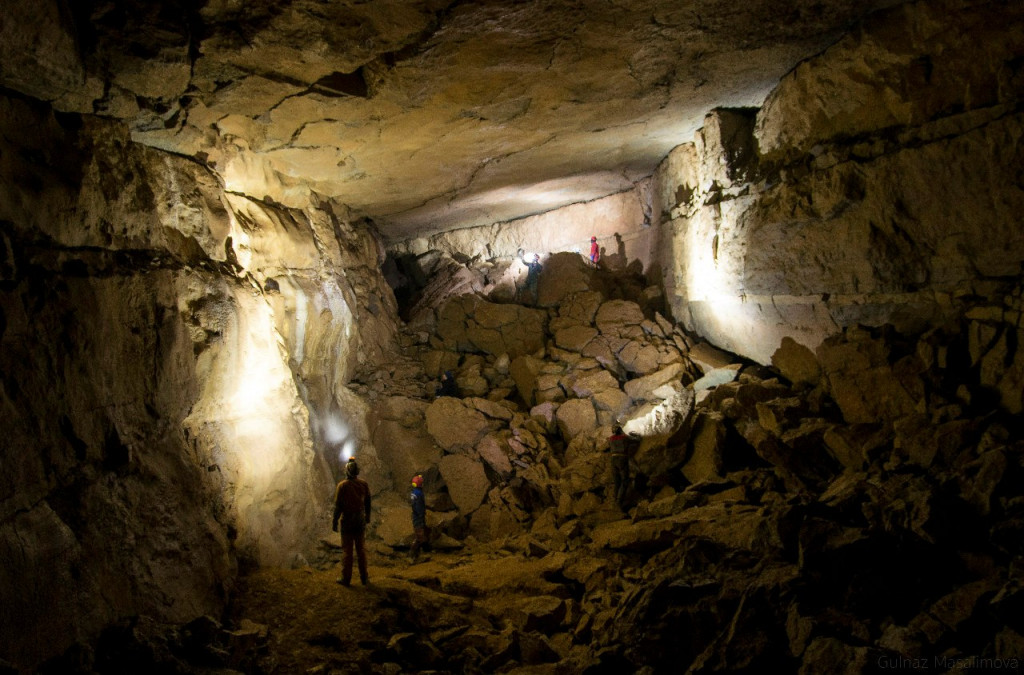
\includegraphics[height=1.75cm,width=1\textwidth,keepaspectratio]{../images/slides/rip.jpg}
                    \caption*{Завал}
                \end{subfigure}
                \begin{subfigure}{0.49\textwidth}
                    \centering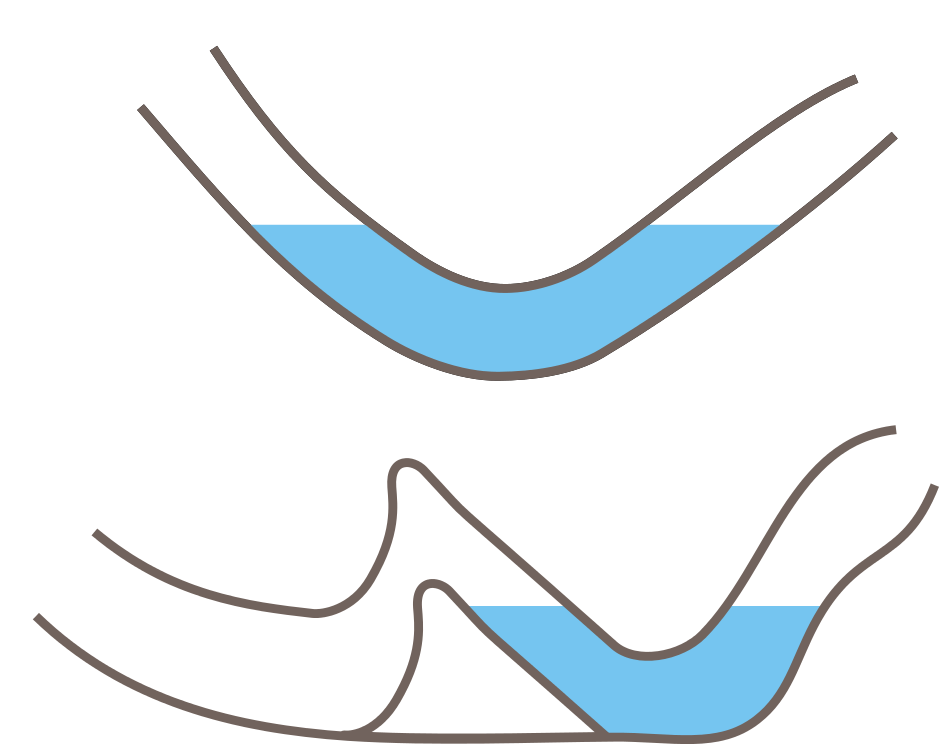
\includegraphics[height=1.75cm,width=1\textwidth,keepaspectratio]{../images/surface_types/siphon.png}
                    \caption*{Сифоны}
                \end{subfigure}
            
                \begin{subfigure}{0.49\textwidth}
                    \centering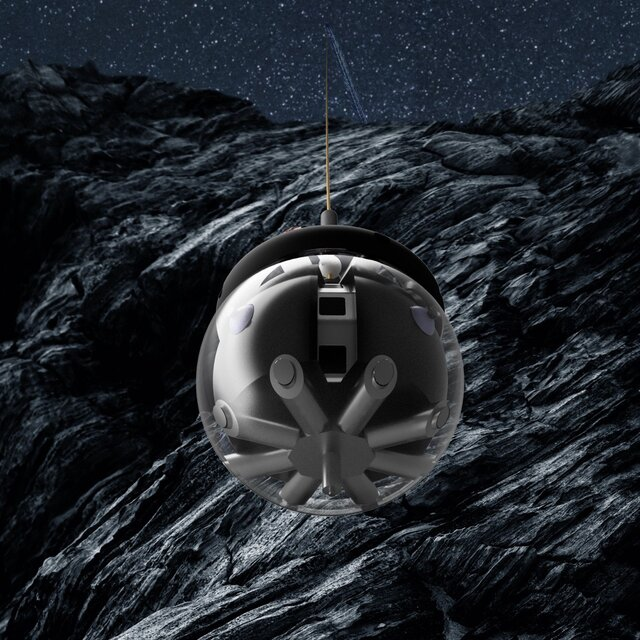
\includegraphics[height=2cm,width=1\textwidth,keepaspectratio]{../images/slides/daedalus.jpg}
                    \caption*{DAEDALUS для исследования пещер на луне}
                \end{subfigure}
                \begin{subfigure}{0.49\textwidth}
                    \centering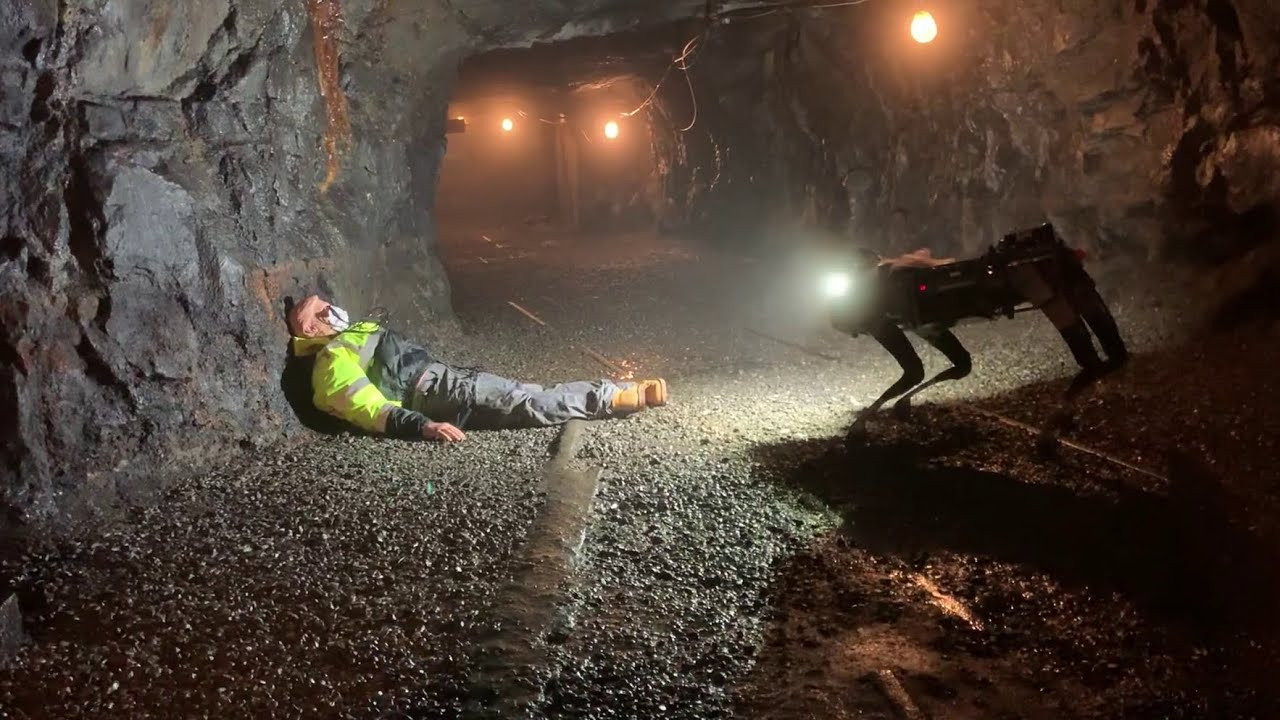
\includegraphics[height=2cm,width=1\textwidth,keepaspectratio]{../images/open_cave.jpg}
                    \caption*{DARPA Subterranean Challenge}
                \end{subfigure}
            \end{figure}
        \end{column}
    \end{columns}
\end{frame}

\note{
\small \setlength{\parindent}{20pt}
\begin{itemize}
    \item Одним из способов нахождения новых минералов или форм жизни является исследование пещер спелеологами. Но данное мероприятие очень опасно, так как
    \item Поэтому разные организации во всем мире пытаются начать применять роботов при исследовании пещер
\end{itemize}  
 }

\begin{frame}[t]{Характеристики пещер}
    \framesubtitle{}
    \vspace{-0.8cm}
    \begin{figure}[H]
        \begin{subfigure}{0.49\textwidth}
            \begin{subfigure}[b]{0.49\textwidth}
                \centering\includegraphics[height=2.2cm,width=1\textwidth,keepaspectratio,page=1]{./tikz_pictures.pdf}
                \caption{Малый водоем}
            \end{subfigure}
            \hfill
            \begin{subfigure}[b]{0.49\textwidth}
                \centering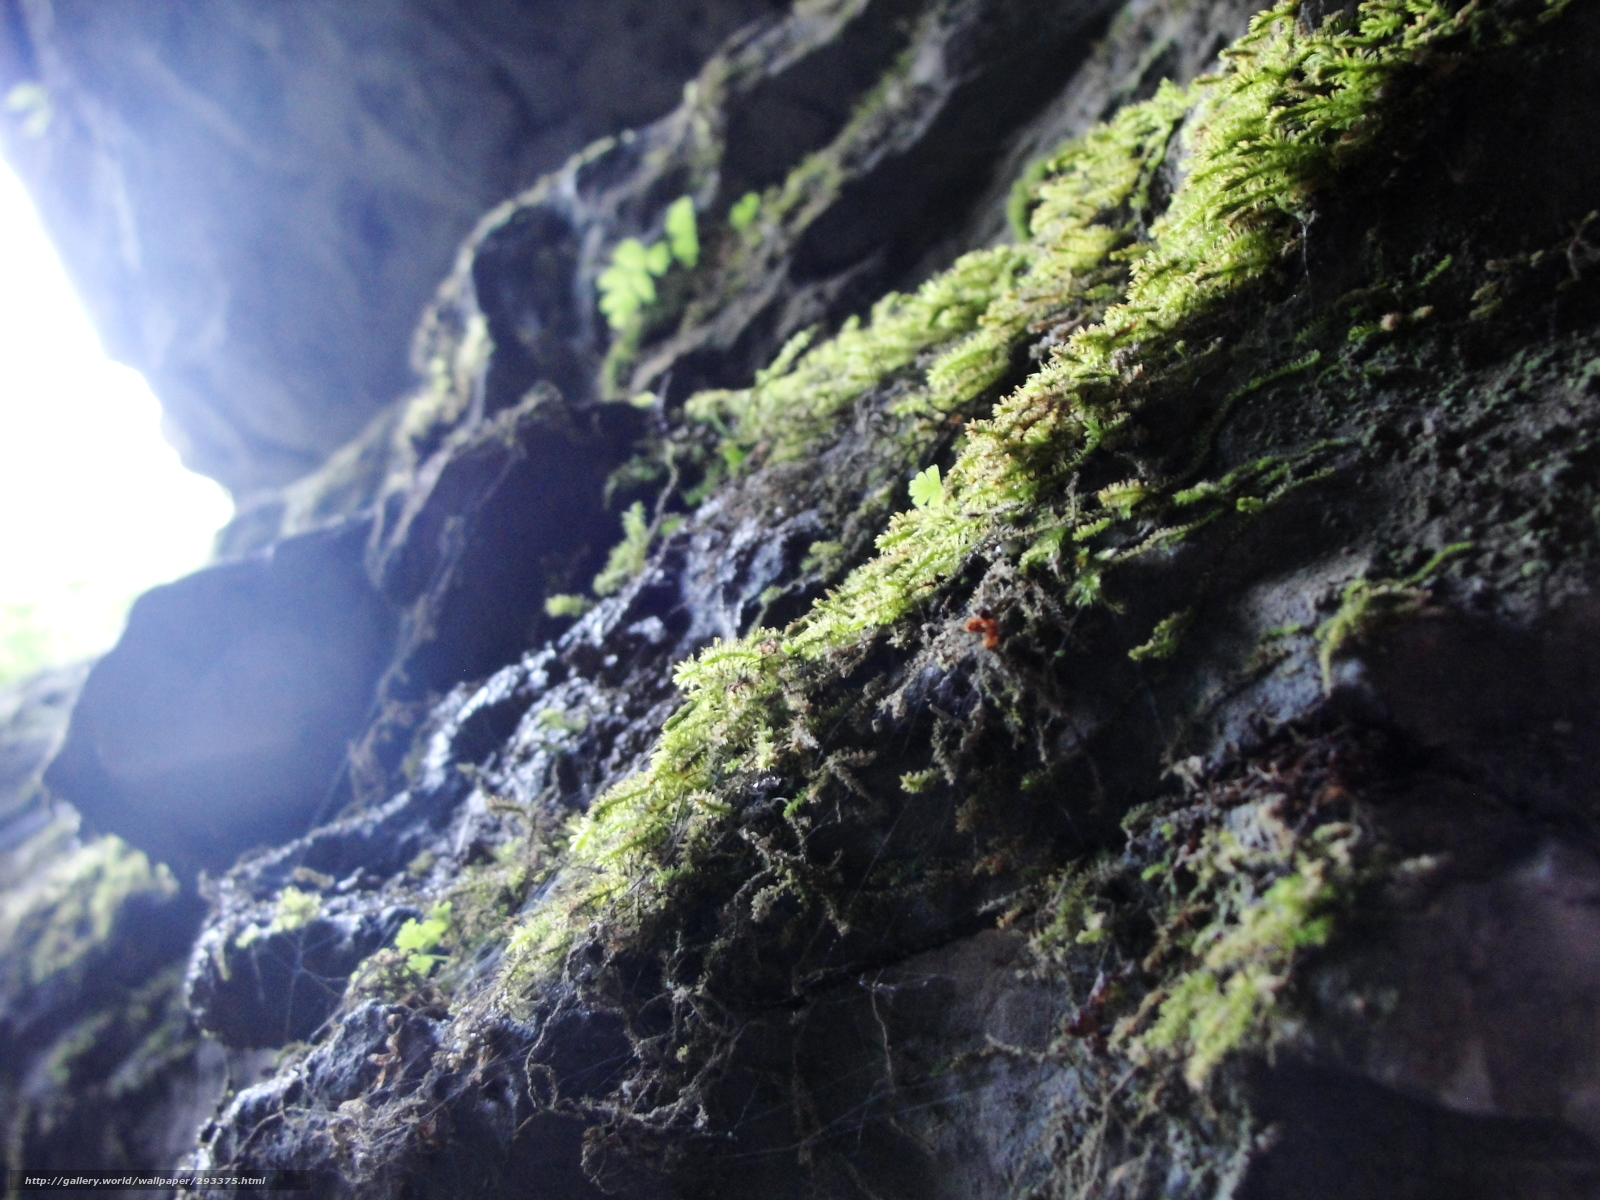
\includegraphics[height=2.2cm,width=1\textwidth,keepaspectratio]{surface_types/moss.jpg}\\
                \caption{Мох}
            \end{subfigure}

            \begin{subfigure}[b]{0.49\textwidth}
                \centering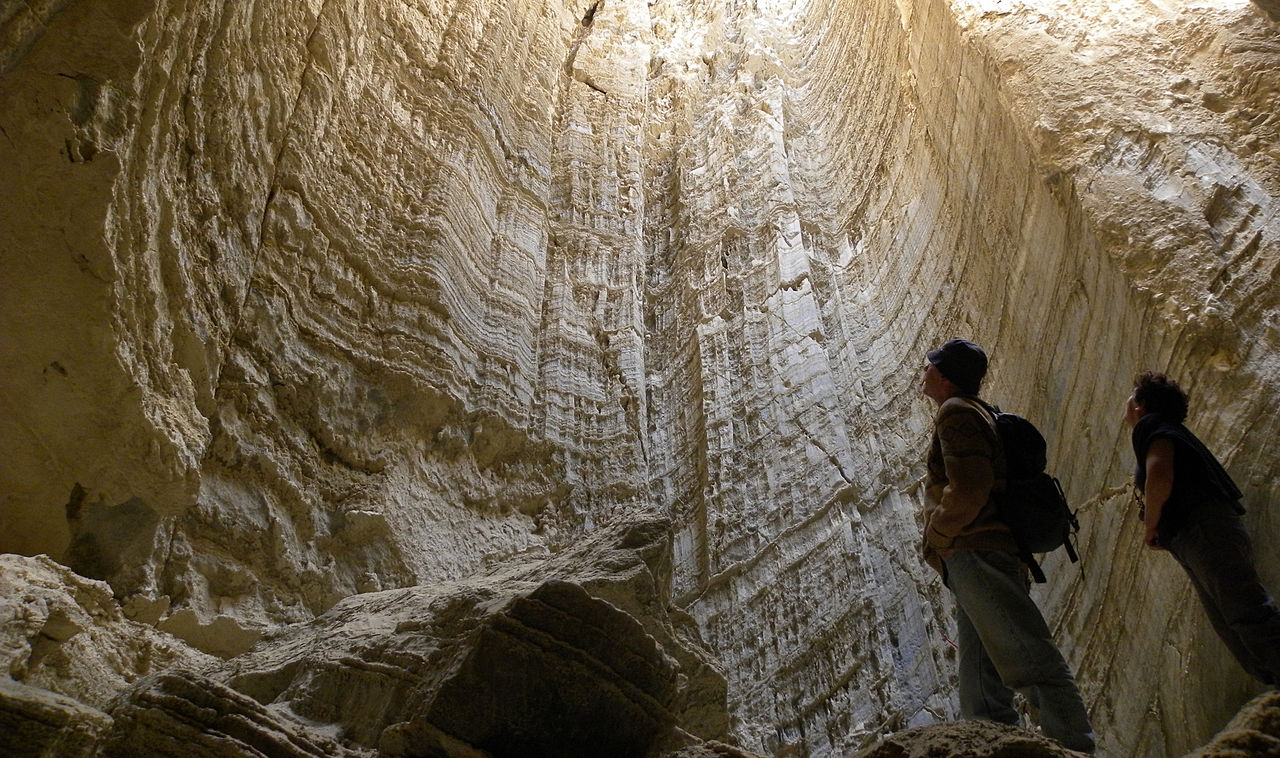
\includegraphics[height=2.0cm,width=1\textwidth,keepaspectratio]{surface_types/salt.jpg}\\
                \caption{Твердые породы}
            \end{subfigure}
            \begin{subfigure}[b]{0.49\textwidth}
                \centering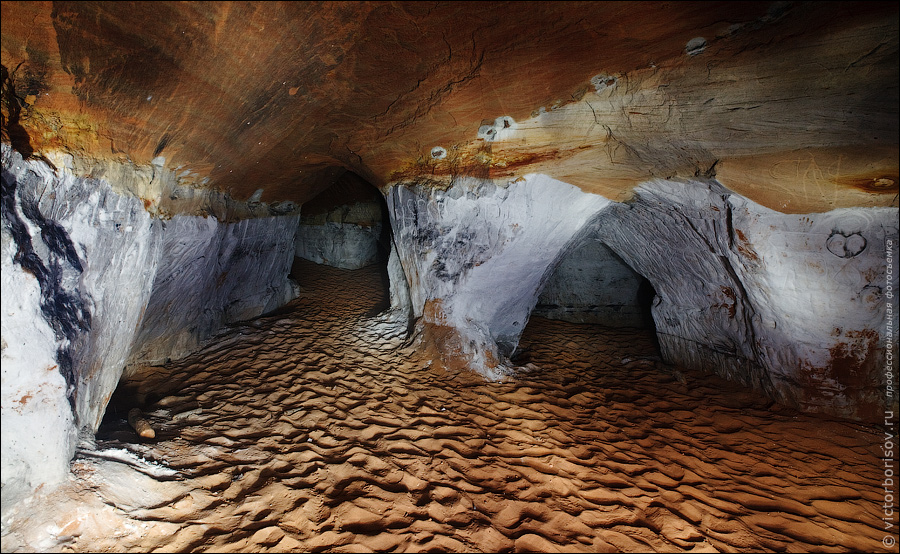
\includegraphics[height=2.0cm,width=1\textwidth,keepaspectratio]{surface_types/sand.jpg}\\
                \caption{Грунт}
            \end{subfigure}
            \caption*{Типы опорных поверхностей}
        \end{subfigure}
        \begin{subfigure}{0.49\textwidth}
            \begin{subfigure}{0.99\textwidth}
                \centering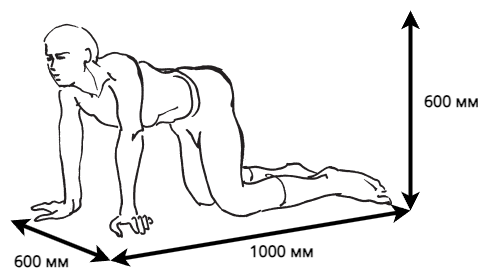
\includegraphics[height=3cm,width=1\textwidth,keepaspectratio]{../images/human_crawling.png}
                \caption*{Габариты пещеры (Свободная узость)}
            \end{subfigure}

            \begin{subfigure}{0.99\textwidth}
                \centering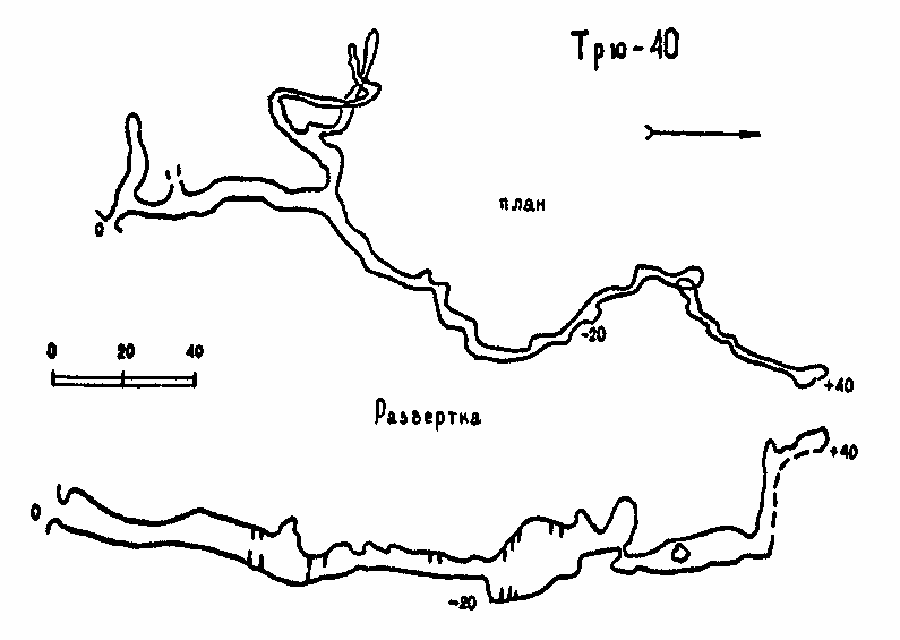
\includegraphics[height=3cm,width=1\textwidth,keepaspectratio]{../images/cave_maps/map3.png}
                \caption*{Протяженность пещер: 1--2 км}
            \end{subfigure}
        \end{subfigure}
    \end{figure}
\end{frame}

\note{\small \setlength{\parindent}{20pt}
\begin{itemize}
    \item Так как пещеры бывают абсолютно разными, я решил ограничить спектр пещер для которых решалась задача. Слева представлены типы опорных поверхностей
    \item Для разработки объекта исследования необходимо понимать также и габариты пещер, а также их протяженность
    \item Глобальная миссия --- разработать робота для исследования пещер.
\end{itemize}
}

% \begin{frame}[t]{Некорректные данные с оптических сенсоров}
%     \framesubtitle{}
%     \begin{figure}[H]
%         \begin{subfigure}[t]{0.49\textwidth}
%             \centering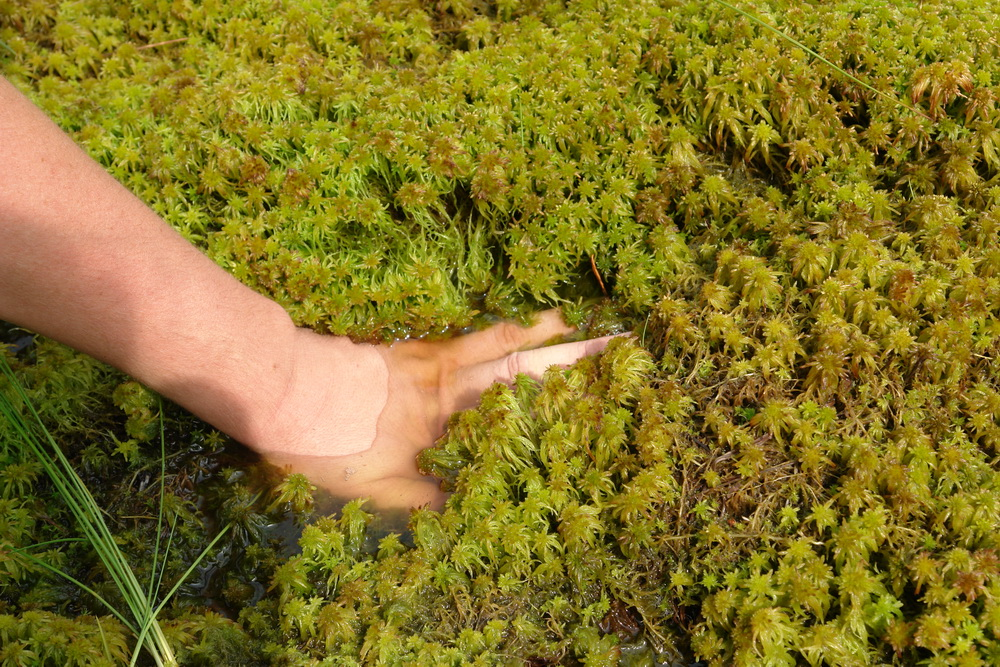
\includegraphics[height=5cm,width=1\textwidth,keepaspectratio]{../images/moh_damping.jpg}
%             \caption*{Мох приминается после ходьбы}
%         \end{subfigure}
%         \begin{subfigure}[t]{0.49\textwidth}
%             \centering\includegraphics[height=5cm,width=1\textwidth,keepaspectratio,page=2]{./tikz_pictures.pdf}
%             \caption*{Лазер отражается от воды, а камера не различает объекты в мутной воде}
%         \end{subfigure}
%     \end{figure}
% \end{frame}

% \note{\small \setlength{\parindent}{20pt}
% Для исследования пещер роботу нужна система навигации. Классические системы навигации основаны на оптических сенсорах.

% К сожалению, в пещерах встречаются случаи, когда оптические сенсоры: лидары, камеры, не смогут достоверно построить карту.

% К примеру, мох *тык*. Он меняет свой объем при наступании на него и это возможно только измерить во время ходьбы. До или после будут уже другой рельеф. 

% Второй пример --- построение опорной поверхности под лужей *тык*. Лидар будет отражаться от поверхности воды и построит гладкую поверхность, а камера не будет работать в мутной воде, как и зеленый лидар.

% С использованием же разработанных методов, данная задача решаема, что и будет показано далее.
% }

\begin{frame}[t]{Цель работы}
    \framesubtitle{}
    Разработать \textbf{метод построения карты местности} с определением \underline{геометрических} и \underline{физико-механических} свойств \textit{опорной поверхности} роботом с шагающими движителями снабженными \underline{тактильными датчиками}, \textit{без использования оптических сенсоров}.
    \begin{figure}[H]
        \begin{subfigure}{0.49\textwidth}
            \centering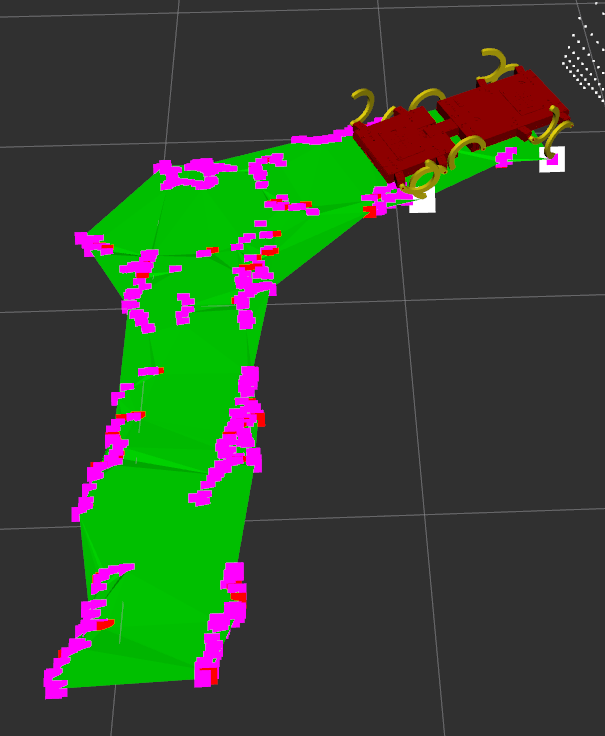
\includegraphics[height=4cm,width=1\textwidth,keepaspectratio]{../images/slides/geom_prop.png}
            \caption*{Определение геометрических свойств}
        \end{subfigure}
        \begin{subfigure}{0.49\textwidth}
            \centering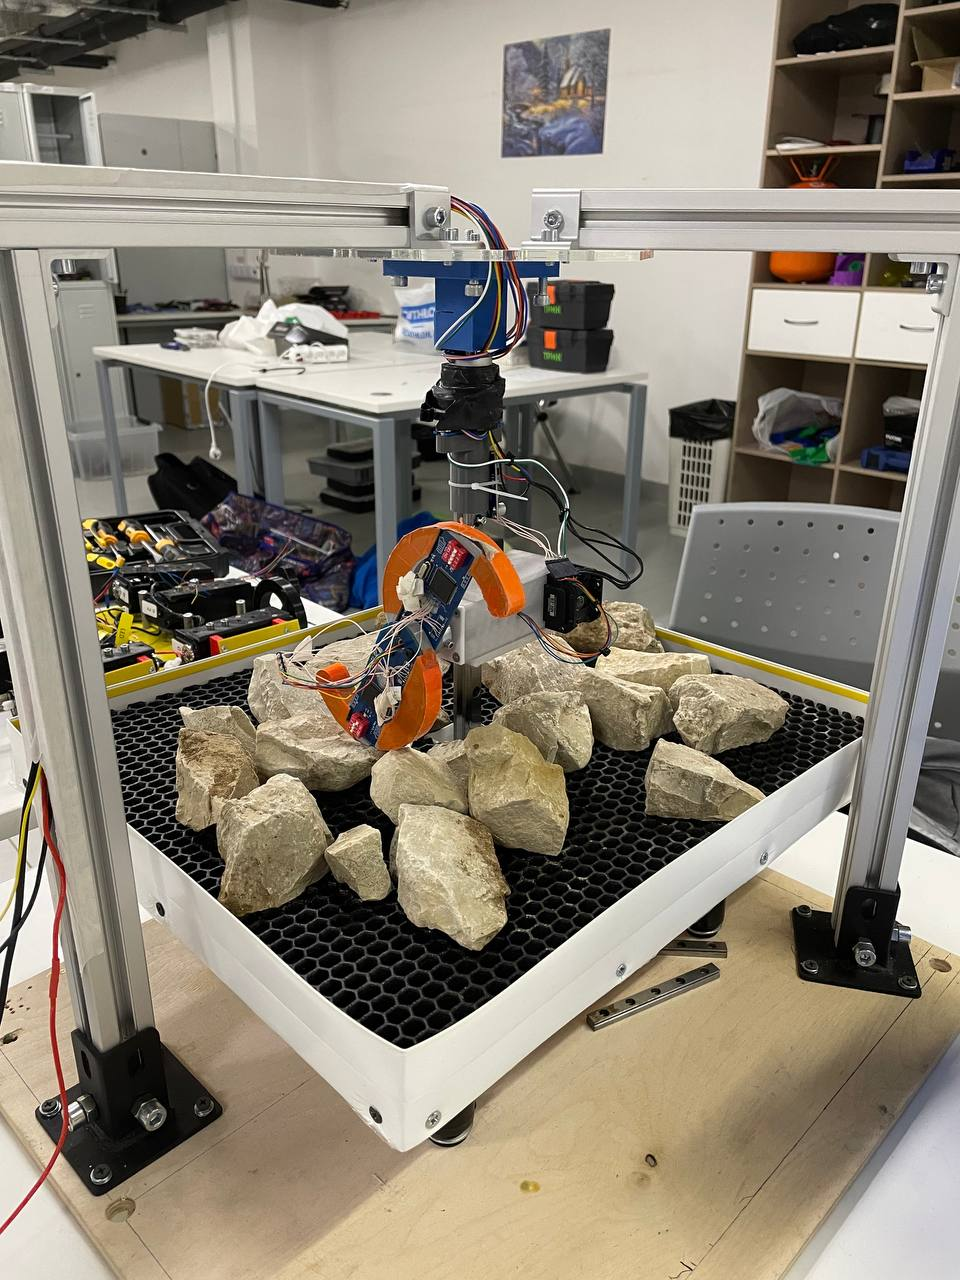
\includegraphics[height=4cm,width=1\textwidth,keepaspectratio]{s_shape_leg/view.jpg}
            \caption*{Определение физических свойств}
        \end{subfigure}
    \end{figure}
\end{frame}

\note{\small \setlength{\parindent}{20pt}
Целью работы являлось разработать метод построения карты местности роботом с шагающими движителями, у которого на стопах установлены датчики силы. Задача должна решаться без использования оптических сенсоров.

Я разбил понятие построения карты на две задачи: определение геометрических свойств *тык* и физико - механических *тык*.

}

\begin{frame}[t]{Построение рельефа местности}
    \framesubtitle{}
    \begin{columns}[T,onlytextwidth]
        \begin{column}{0.49\textwidth}
            \textbf{"4" Геометрические свойства}\\
            \textit{Входные данные}: следовая дорожка, представленная в виде облака точек.

            \textit{Выходные данные}: полигональная сетка и плотное облако точек.
            \vspace{0.35cm}
            \begin{figure}[H]
                \begin{subfigure}[t]{0.49\textwidth}
                    \centering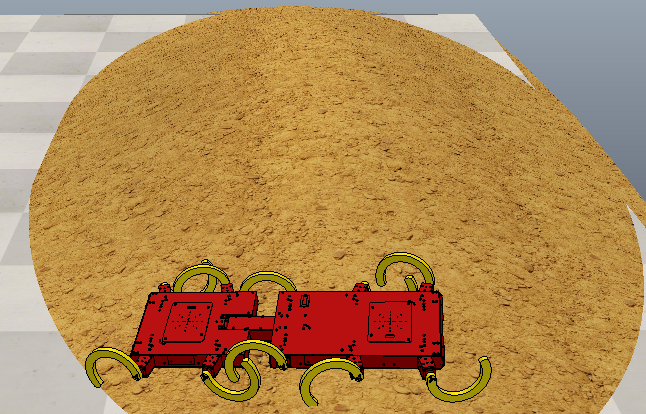
\includegraphics[height=1.9cm,width=1\textwidth,keepaspectratio]{../images/slides/surface_research.png}
                    \caption*{Исследуемая поверхность}
                \end{subfigure}
                \begin{subfigure}[t]{0.49\textwidth}
                    \centering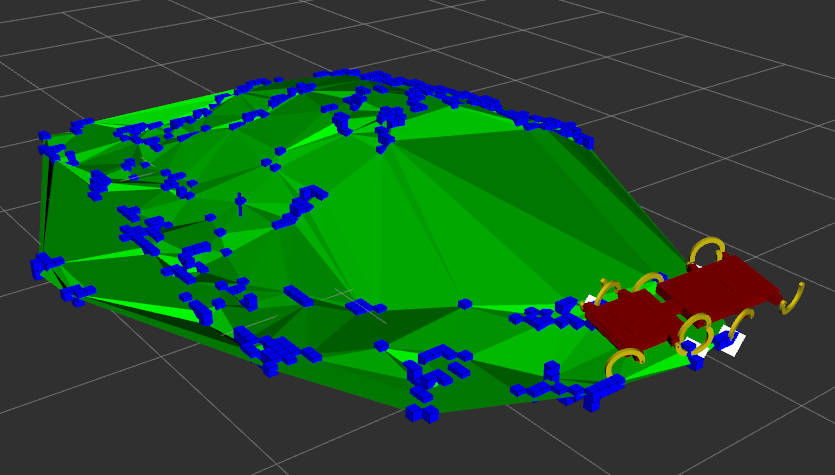
\includegraphics[height=1.9cm,width=1\textwidth,keepaspectratio]{../images/slides/result_research.png}
                    \caption*{Следовая дорожка и полигональная сетка}
                \end{subfigure}
            \end{figure}
        \end{column}
        \begin{column}{0.49\textwidth}
            \textbf{"3" Физико-механические свойства}\\
            \textit{Входные данные}: данные с внутренних датчиков робота.

            \textit{Выходные данные}: процентное соотношение упругих, твердых и пластичных свойств пройденной поверхности.

            \vspace{-0.35cm}
            \begin{figure}[H]
                \begin{subfigure}[t]{0.49\textwidth}
                    \centering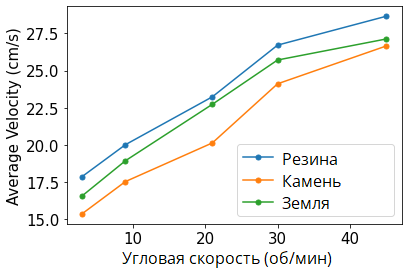
\includegraphics[height=2.5cm,width=1\textwidth,keepaspectratio]{../images/slides/avg_lin_vel_rev_min.png}
                    \caption*{Данные для обучения}
                \end{subfigure}
                \begin{subfigure}[t]{0.49\textwidth}
                    \centering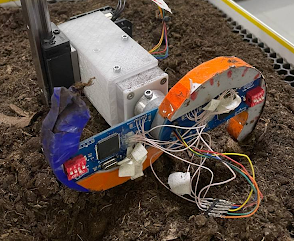
\includegraphics[height=2.5cm,width=1\textwidth,keepaspectratio]{../images/slides/data.png}
                    \caption*{Пример поверхности}
                \end{subfigure}
            \end{figure}
        \end{column}
    \end{columns}
\end{frame}

\note{\small \setlength{\parindent}{20pt}
\begin{itemize}
    \item Задача 4 --- Результатом примененного метода решения должны получиться полигональная сетка пройденной исследуемой поверхности
    \item Задача 3 --- определение какие свойства у пройденной поверхности превалируют: твердые, упругие или пластичные. То есть не всех свойств, а только некоторых
\end{itemize}}

\begin{frame}[t]{Основные научные задачи исследования}
    \framesubtitle{}
    \begin{enumerate}
        \item Разработка метода \textbf{оптимизации конструкции многоногих шагающих роботов} с цикловыми движителями с одной степенью свободы по критериям проходимости, покрытия опорной поверхности и её детализации, длины пройденного пути.
        \item Создание методики \textbf{исследования датчика силы}, когда площадь контакта нажатия на сенсор меньше чувствительной области самого сенсора.
        \item Реализация алгоритма, позволяющего \textbf{определять физические свойства} опорной поверхности.
        \item  Разработка метода \textbf{построения карты местности и определения геометрических свойств поверхности} с помощью тактильного очувствления.
    \end{enumerate}
\end{frame}

\note{\small \setlength{\parindent}{20pt}
\begin{itemize}
    \item Но для решения основных задач, необходимо вначале создать робота и его оптимизировать
    \item Создать датчик и его исследовать
\end{itemize}
}


\begin{frame}{Положения, выносимые на защиту}
    \begin{enumerate}
        \vspace{-0.3cm}
        \small
        \item \textbf{Метод определения физико-механических свойств опорной поверхности} на основе \textbf{тактильного очувствления}, позволяющий различать материалы с \textit{упругими, жёсткими, пластичными свойствами}.
        \item \textbf{Метод построения карты местности}, состоящий в определении геометрической формы поверхности с помощью тактильного очувствления, который позволяет решать задачу определения плана и профиля поверхности в условиях отсутствия видимости и при движении по поверхности, находящейся под водой.
        \item \textbf{Критерий оптимизации} кинематической схемы многоногих шагающих роботов с цикловыми одностепенными движителями, включающий в себя показатели проходимости, покрытия опорной поверхности и её детализации. Определение на его основе габаритов и количества движителей шагающего робота.
        \item \textbf{Зависимость} \textit{погрешности} датчика силы на основе полимерного материала от \textit{площади пятна контакта} относительно размеров датчика, применяемого для тактильного очувствления мобильного робота. \textbf{Методика} роботизированного исследования датчика силы.
    \end{enumerate}
\end{frame}

\note{\small \setlength{\parindent}{20pt}

На защиту выносятся 2 метода, зависимость и критерий оптимизации кинематической схемы}

\begin{frame}[t]{Объект исследования}
    \framesubtitle{}
    \begin{columns}[T,onlytextwidth]
        \begin{column}{0.49\textwidth}
            \textbf{Класс многоногих шагающих роботов} с \\
            а) \underline{Цельным} или \underline{сочленённым} \textit{корпусом}\\
            б) \underline{Цикловыми} \textit{движителями} с \underline{одной степенью свободы}, управляемые зависимо или независимо друг от друга.

            \textit{Требования}:
            \begin{itemize}
                \item Компактные размеры (меньше чем $1000\times600\times600$ мм)
                \item Залезать на препятствия высотой не меньше, чем $\frac{3}{4}$ длины корпуса
                \item Преодолевать представленные
                      опорные поверхности
            \end{itemize}
        \end{column}
        \begin{column}{0.49\textwidth}
            \begin{figure}[H]
                \hfill
                \begin{subfigure}{0.99\textwidth}
                    \centering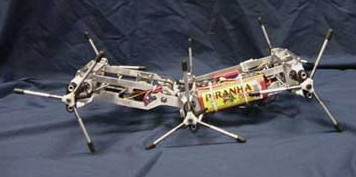
\includegraphics[height=2.5cm,width=1\textwidth,keepaspectratio]{from_master/whegs2.jpg}
                    \caption*{WHegs}
                \end{subfigure}

                \hfill
                \begin{subfigure}[t]{0.49\textwidth}
                    \centering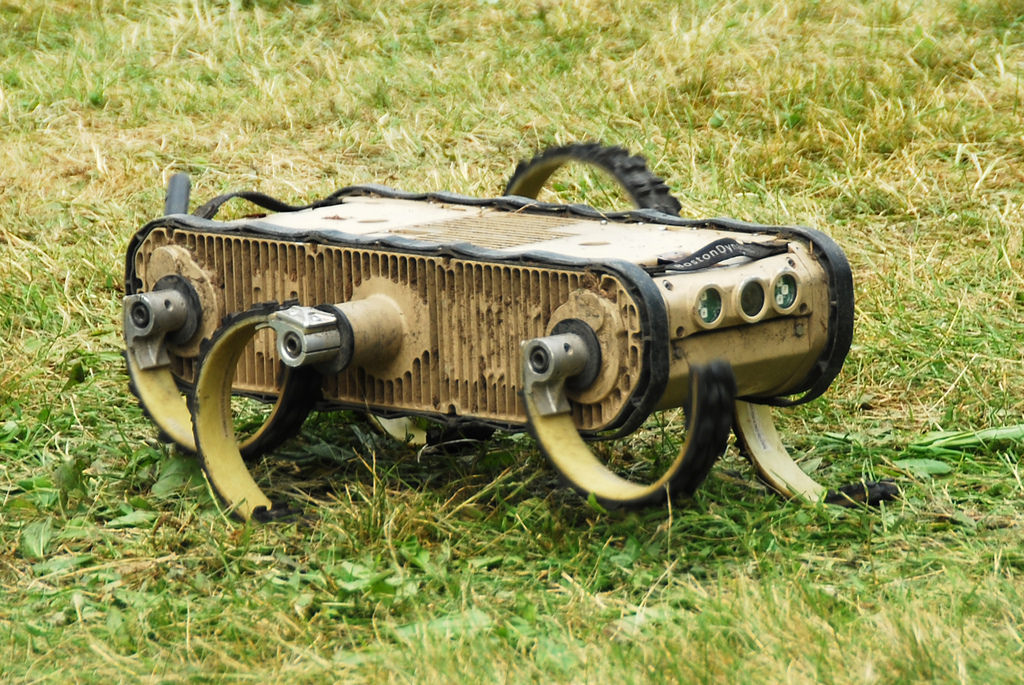
\includegraphics[height=2.5cm,width=1\textwidth,keepaspectratio]{from_master/rhex.jpg}
                    \caption*{Boston Dynamics RHex}
                \end{subfigure}
                \begin{subfigure}[t]{0.49\textwidth}
                    \centering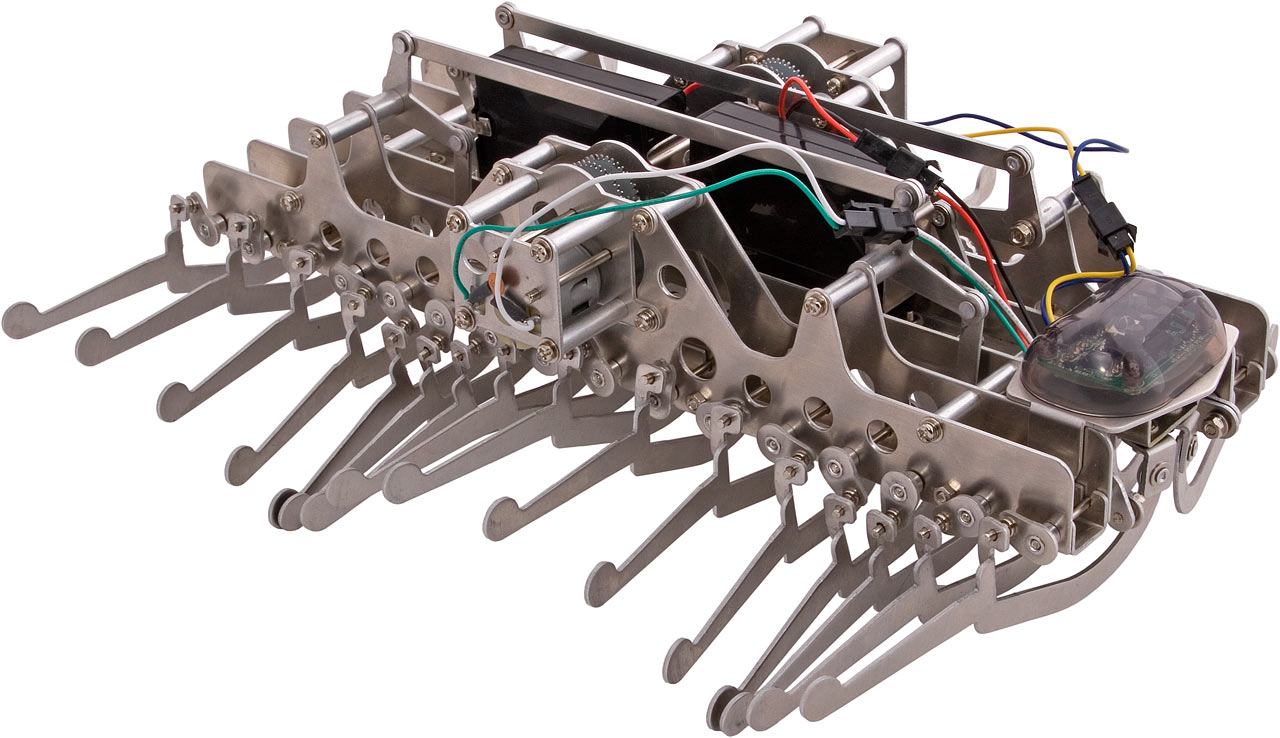
\includegraphics[height=2.5cm,width=1\textwidth,keepaspectratio]{from_master/gakken.jpg}
                    \caption*{Gakken Centipede}
                \end{subfigure}
            \end{figure}
        \end{column}
    \end{columns}
\end{frame}

\note{\small \setlength{\parindent}{20pt}
\begin{itemize}
    \item На основе описания характеристик пещер, мной были выдвинуты требования к объекту исследования
    \item Рассмотрев различные варианты кинематических схем,
    \item В данном видео видно, как подобный класс ...
\end{itemize}
}

\section{Обзор существующих решений}

\begin{frame}[t]{Структура робота}
    \framesubtitle{}
    \begin{figure}[H]
        \centering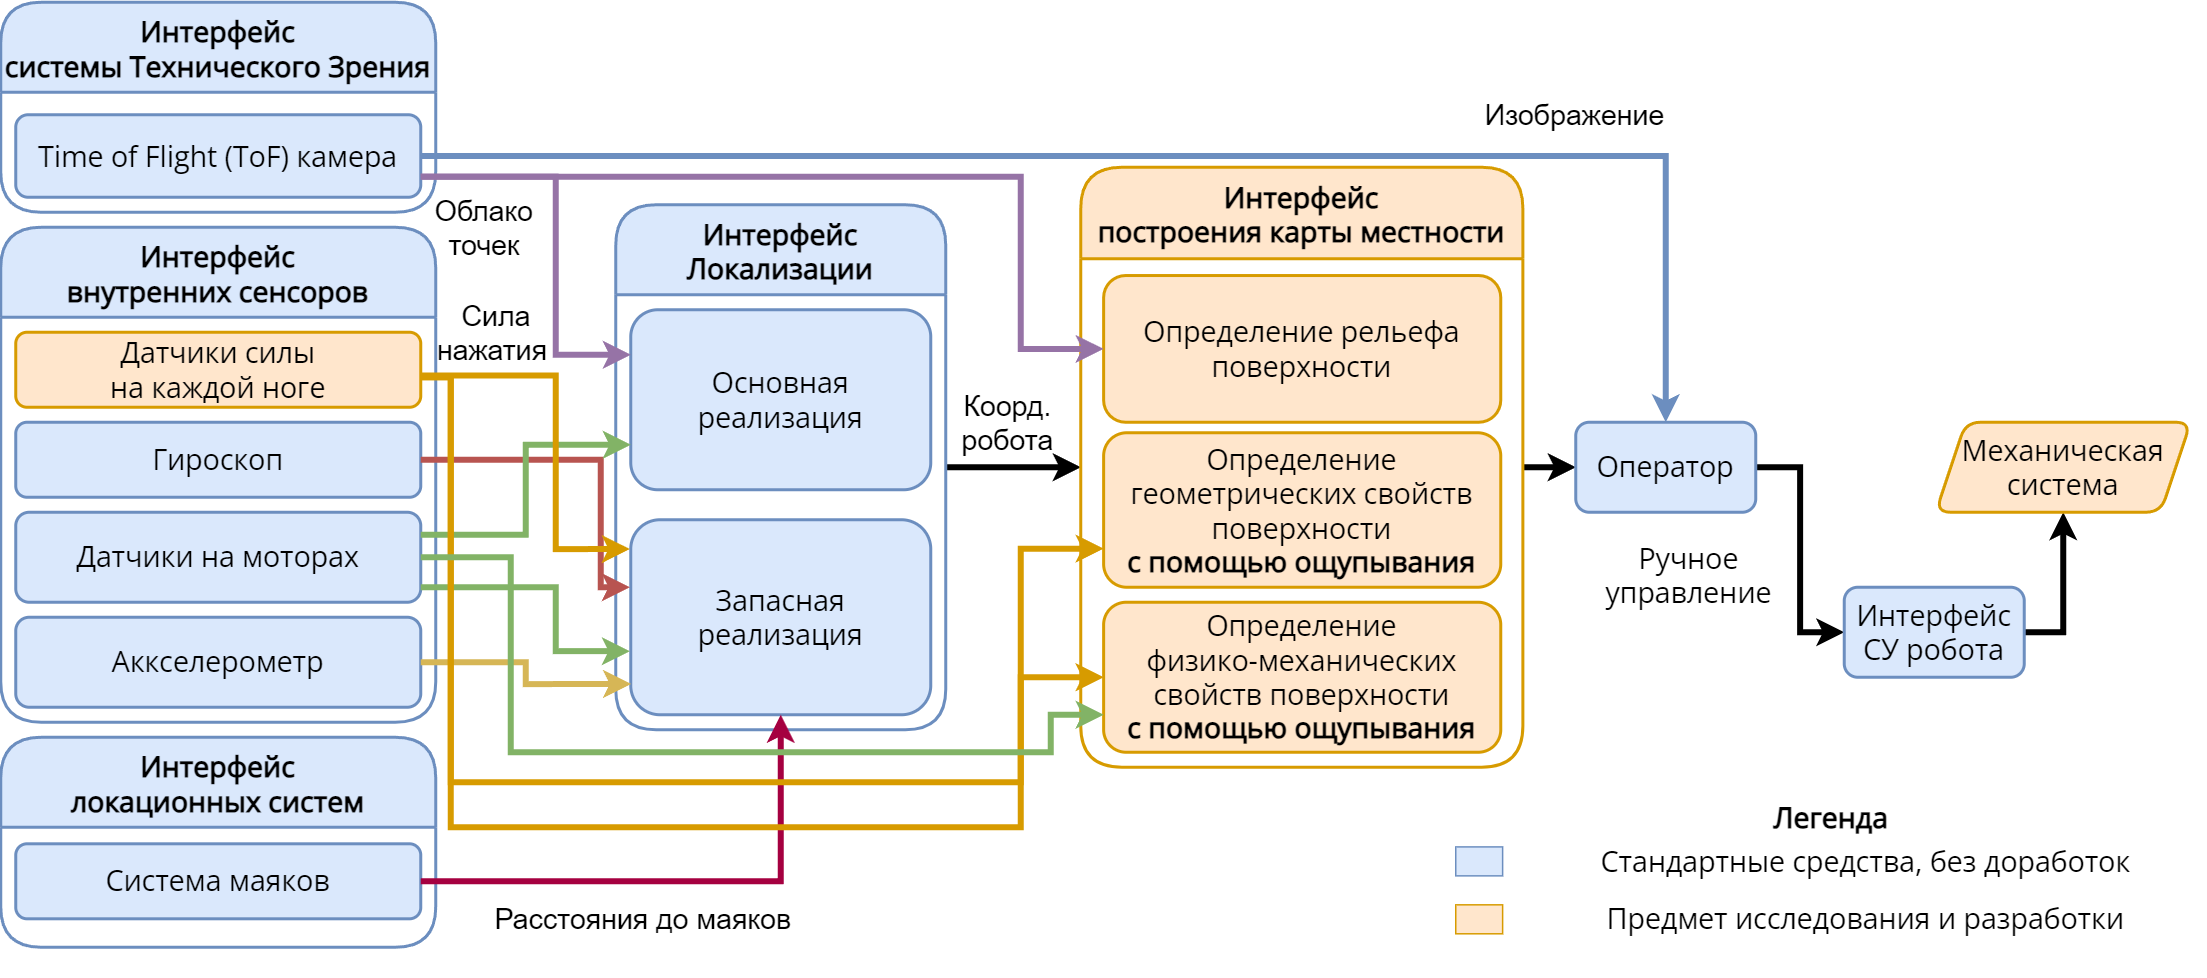
\includegraphics[height=6.5cm,width=1\textwidth,keepaspectratio]{main_diag_hor_new.png}
    \end{figure}
\end{frame}

\note{\small \setlength{\parindent}{20pt}
\begin{itemize}
    \item Робот --- сложная система с множеством подсистем и большую часть подсистем я сам лично не делал.
    \item На слайде *тык* представлена структура проекта
\end{itemize}
}

\begin{frame}[t]{Обзор источников}
    \framesubtitle{}
    \begin{itemize}
        \item \textbf{Задача оптимизации конструкции}: Б. Петриашвили (СССР), Stefano Nolfi (Италия), Dario Sanch-Pradel (Италия), S. Feng (США) и др.
        \item \textbf{Шагающие цикловые роботы}: Е. С. Брискин (Россия), Ю. Д. Андриантов (СССР), Edward Z. Moore (Канада), Wei-Hsi Chen (Китай) и др.
        \item \textbf{Верификация Velostat}:  Igor Vehec (Словакия),  Robert Schroer (США) и др.
        \item \textbf{Определение геометрических свойств поверхности}: Tobias Ebert (Германия), Subodh Kumar (США), И. Рядчиков (Россия), Shan Luo (Британия) и др.
        \item \textbf{Определение физико-механических свойств поверхности}: X. Alice Wu (США), Krzysztof Walas (Польша), Hendrik Kolvenbach (Швейцария) и др.
    \end{itemize}
\end{frame}

\note{\small \setlength{\parindent}{20pt}
\begin{itemize}
    \item При разработке своих подсистем я базировался на работах следующих ученых со всего мира.
    \item Я изучал источники по всем проблемам, которые я озвучил ранее.
    \item Хочу отметить школу шагающих машин Волгограда, на работах и консультациях которых также базируется мое исследование.
\end{itemize}
}
\section{"1" Оптимизация кинематической схемы}

\begin{frame}[t]{"1" Оптимизация кинематической схемы}
    \framesubtitle{}
    \begin{columns}[T,onlytextwidth]
        \begin{column}{0.45\textwidth}
            Решить задачу оптимизации $F=f(x) \rightarrow max$, где

            $f(x)$ --- критерии: пройденная дистанция, длина корпуса\\
            $(x)$ --- параметры: \textbf{количество ног}, сдвиг фазы между соседними ногами
            \medskip

            \textit{Количество ног имеет прямую зависимость с длиной корпуса робота.}
        \end{column}
        \begin{column}{0.54\textwidth}
            \vspace{-0.5cm}
            \begin{figure}[H]
                \begin{subfigure}{0.99\textwidth}
                    \centering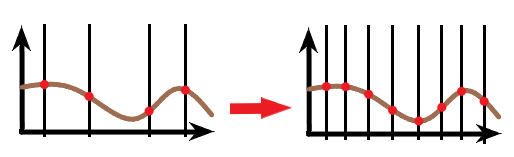
\includegraphics[height=1.8cm,width=1\textwidth,keepaspectratio]{f1.png}
                    \caption*{Кол-во ног $\uparrow$, детализация поверхности $\uparrow$}
                \end{subfigure}

                \begin{subfigure}{0.99\textwidth}
                    \centering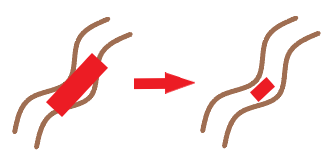
\includegraphics[height=1.8cm,width=1\textwidth,keepaspectratio]{f2.png}
                    \caption*{Длина робота $\uparrow$, курсовая проходимость $\downarrow$}
                \end{subfigure}

                \begin{subfigure}{0.99\textwidth}
                    \centering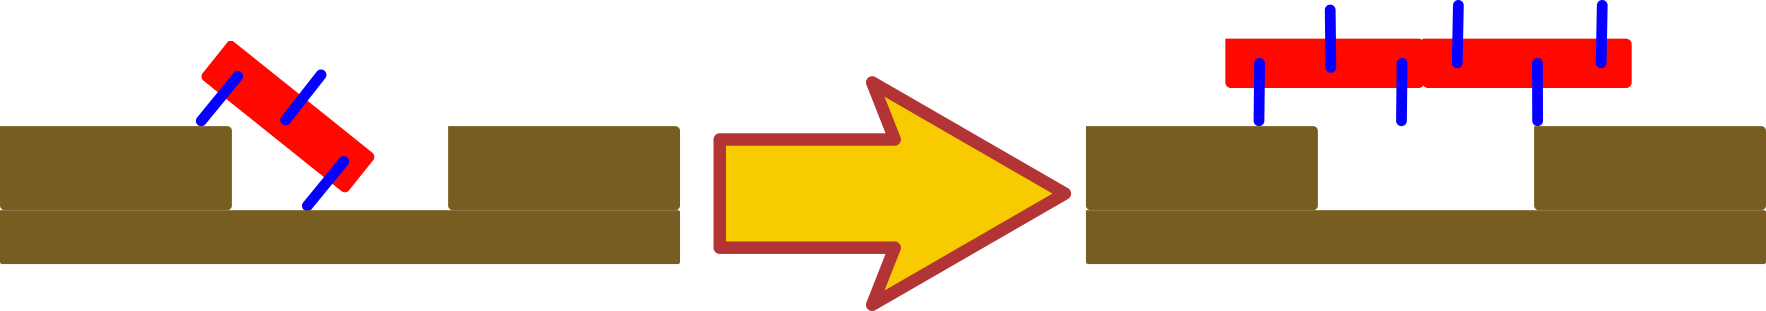
\includegraphics[height=1.8cm,width=1\textwidth,keepaspectratio]{f3_new.png}
                    \caption*{Длина робота $\uparrow$, профильная проходимость $\uparrow$}
                \end{subfigure}
            \end{figure}
        \end{column}
    \end{columns}
\end{frame}

\note{\small \setlength{\parindent}{20pt}
\begin{itemize}
    \item Выбрав кинематическую схему робота, необходимо ее оптимизировать под поставленную задачу, а именно определить количество ног
    \item Чем болше ног ...
    \item То есть я решал мультикритериальную задачу оптимизации, где ...
\end{itemize}
}

\begin{frame}[t]{Определение количества ног}
    \framesubtitle{}
    \begin{columns}[T,onlytextwidth]
        \begin{column}{0.59\textwidth}
            % \small
            % Решить $F=f(x) \rightarrow max$, где

            % $f(x)$ --- \textbf{ Критерии}: пройденная дистанция, длина корпуса\\
            % $x$ --- \textbf{Параметры}: количество ног, сдвиг фазы между соседними ногами

            \textbf{Метод решения}: Генетический алгоритм: Open AI-ES

            \textbf{Алгоритм}: \underline{генерируется множество особей}, а
            также \underline{семейство территорий} с одинаковой сложностью.
            За фиксированное время, с постоянной угловой скоростью
            на моторах, каждый \underline{робот проходит это семейство
            территорий} и записываются данные.

            \textbf{Предположения}: 1) есть только \underline{сухое трение}
            между ногами и поверхностью. 2) Созданные
            поверхности с помощью \underline{одной функции
            и параметров} имеют \underline{одинаковую сложность}.

            \textbf{Утверждение}: \textit{Количество ног имеет прямую
                зависимость с длиной корпуса робота.}
        \end{column}
        \begin{column}{0.39\textwidth}
            \begin{figure}[H]
                \begin{subfigure}{0.49\textwidth}
                    \centering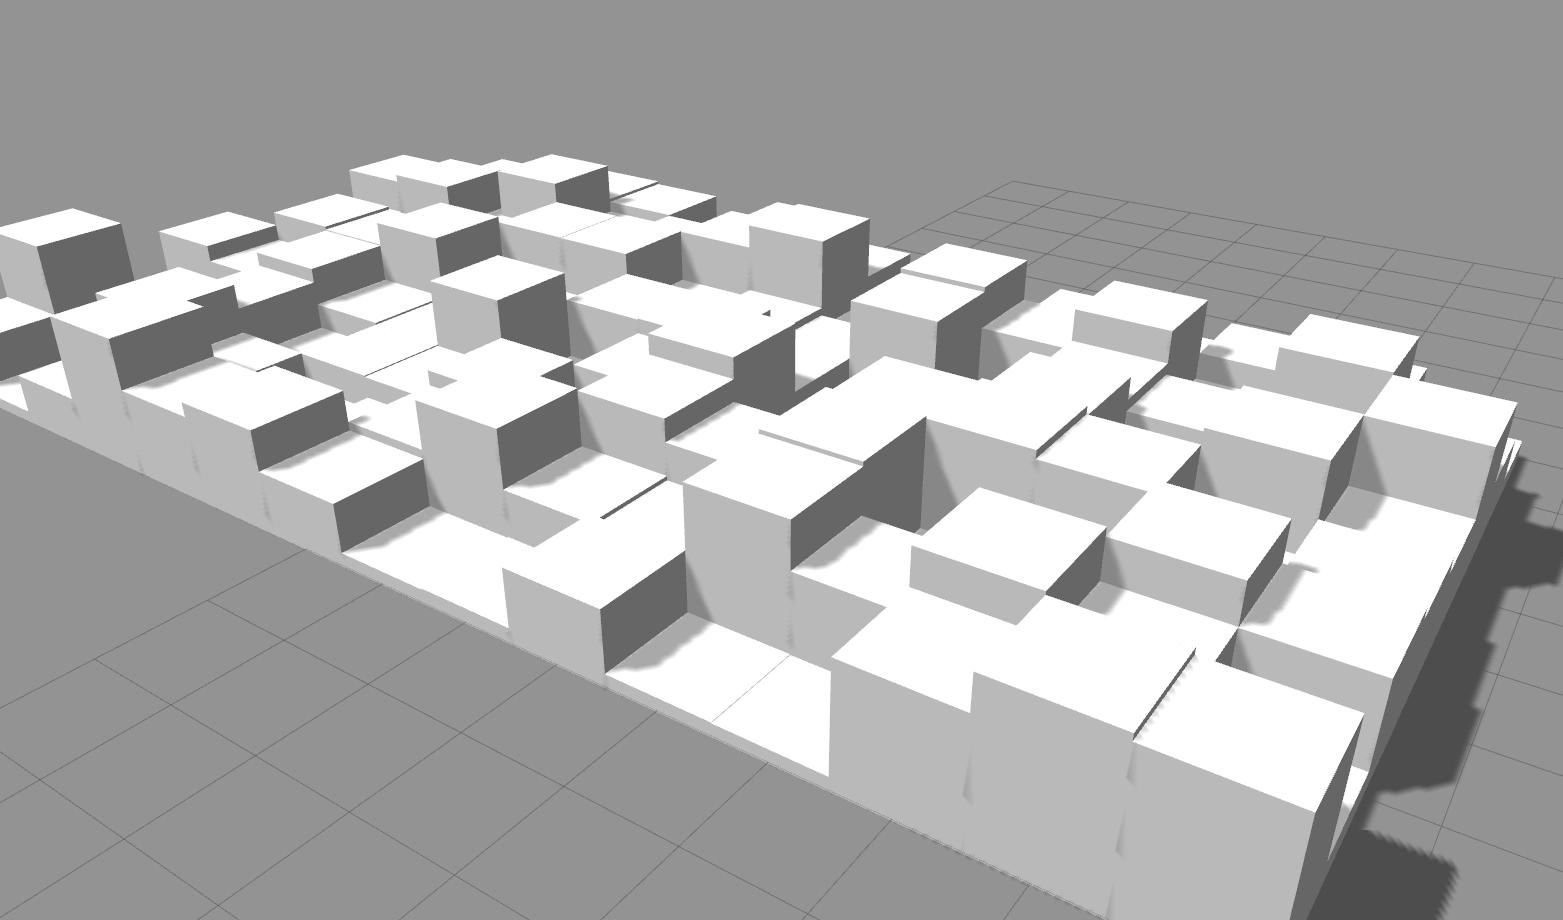
\includegraphics[height=2cm,width=1\textwidth,keepaspectratio]{../images/terrain_1.jpg}
                    \caption*{Равномерное распределение ячеек}
                \end{subfigure}
                \begin{subfigure}{0.49\textwidth}
                    \centering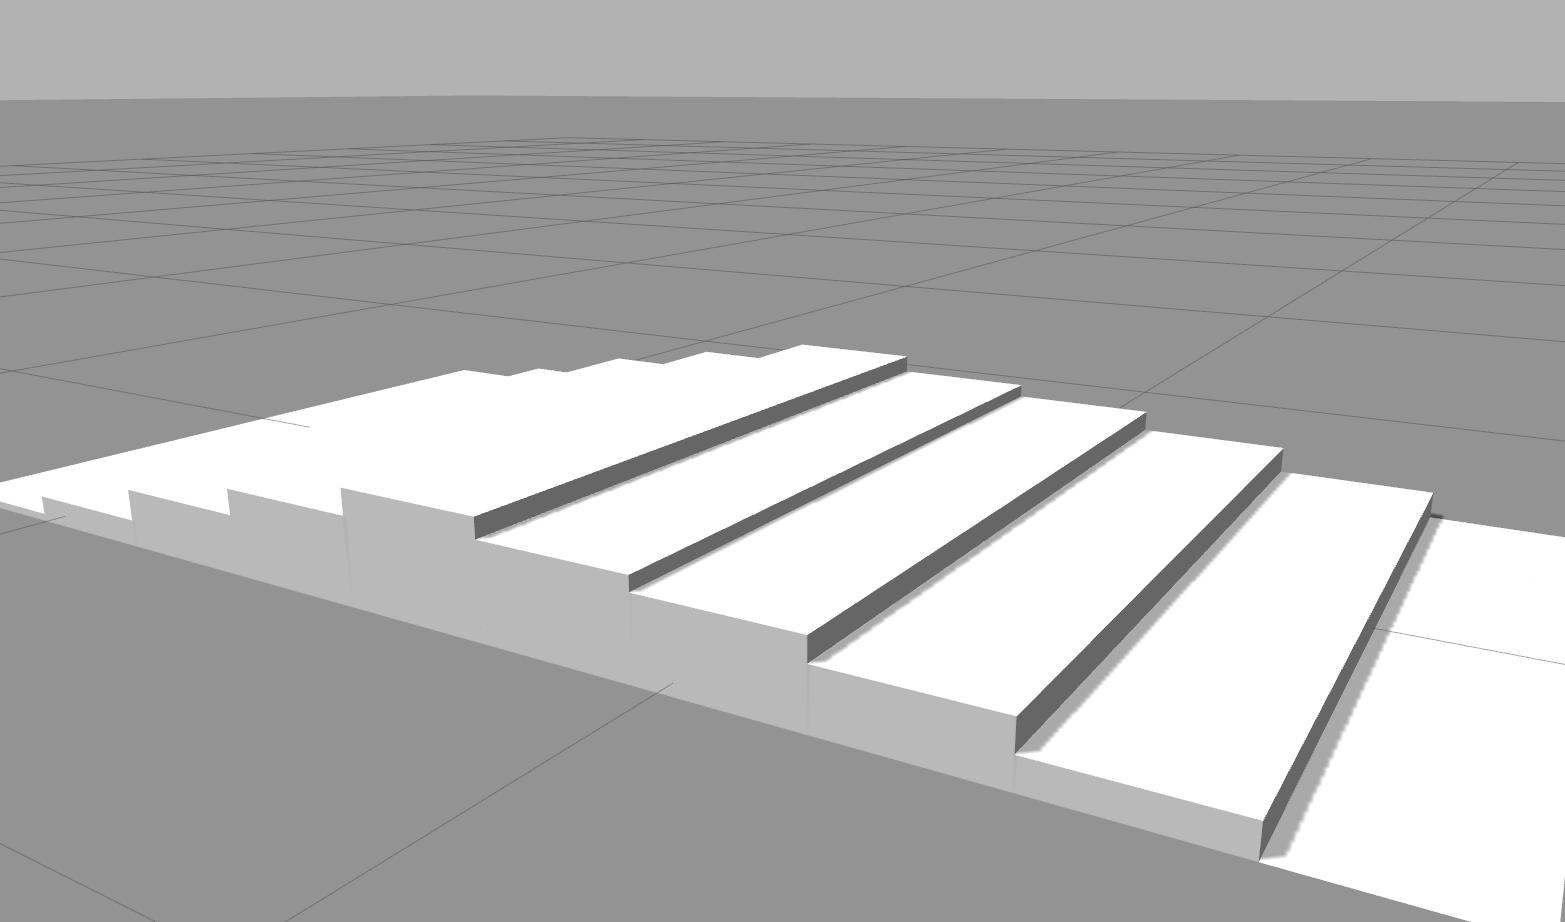
\includegraphics[height=2cm,width=1\textwidth,keepaspectratio]{../images/terrain_2.jpg}
                    \caption*{Гауссово распределение ячеек}
                \end{subfigure}

                \begin{subfigure}{0.99\textwidth}
                    \centering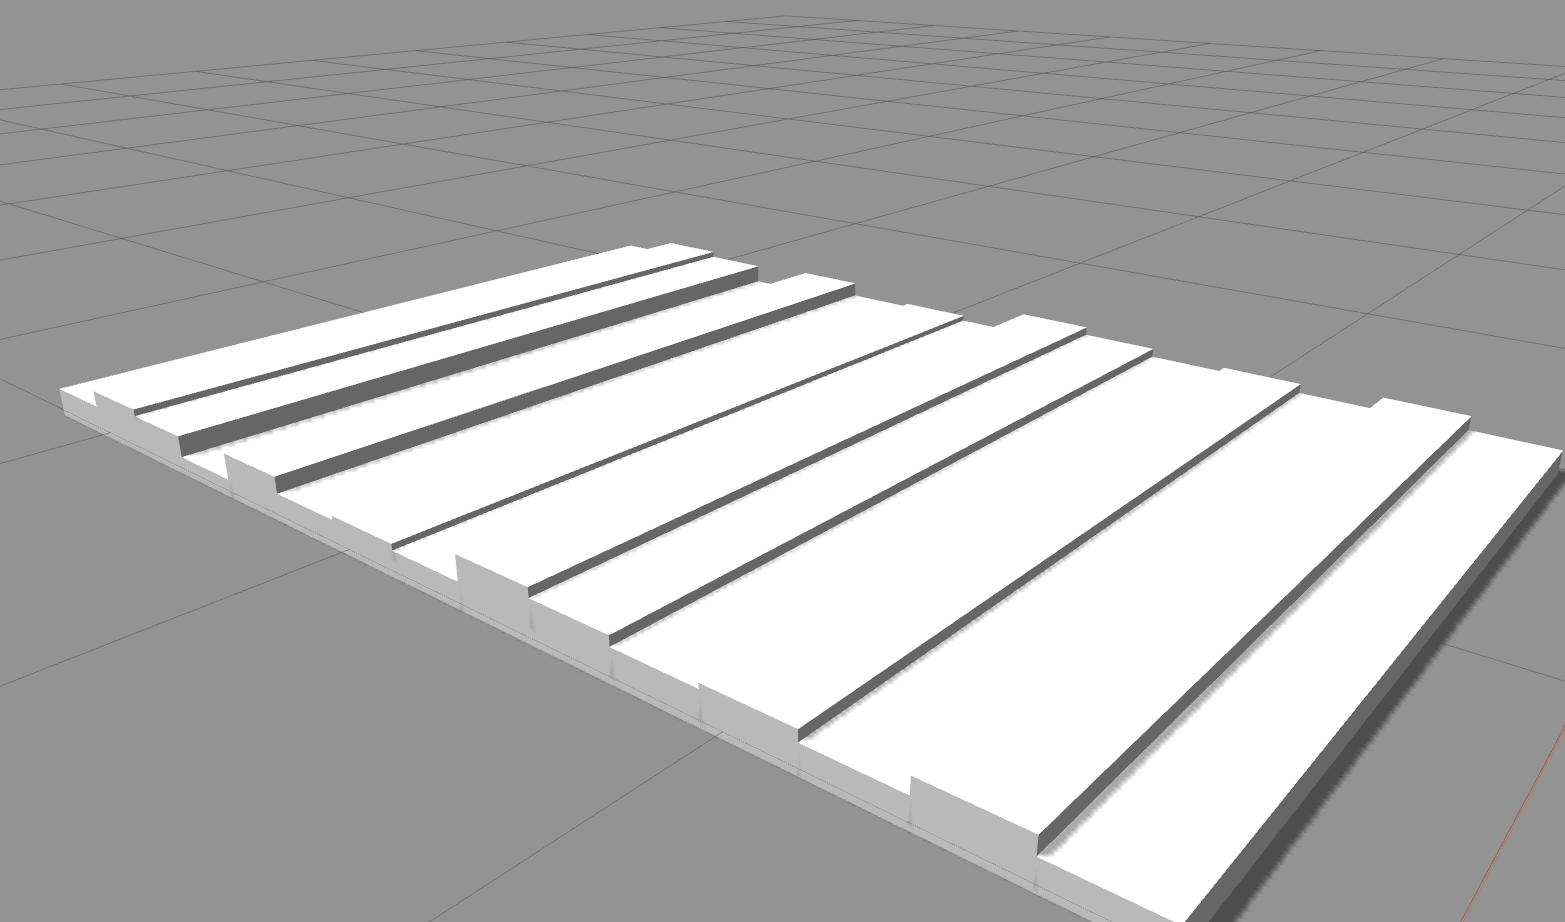
\includegraphics[height=2.8cm,width=1\textwidth,keepaspectratio]{../images/terrain_3.jpg}
                    % \caption*{Пример прохождения особью сгенерированной поверхности}
                \end{subfigure}
            \end{figure}
        \end{column}
    \end{columns}
\end{frame}

\note{\small \setlength{\parindent}{20pt}
\begin{itemize}
    \item Так как я хочу оптимизировать количество ног на основе проходимости, а формализовать территорию является сложной задачей, то было решено решать задачу с помощью генетического алгоритма, где я самостоятельно создавал поверхности с помощью функций распределения.
    \item Примеры территорий и как робот проходит.
\end{itemize}
}



\begin{frame}[t]{Описание механической системы}
    \framesubtitle{}
    \begin{align}
        \boxed{M \dot{\vec{u}} = \vec{g}}                                \\
        M = \begin{bmatrix}
                M_1    & \cdots & 0      \\
                \vdots & \ddots & \vdots \\
                0      & \cdots & M_n
            \end{bmatrix},\ M_i = \begin{bmatrix}
                                      m_i E_{3\times 3} & 0   \\
                                      0                 & I_i
                                  \end{bmatrix}        \\
        \vec{u}_i^{\ T} = \begin{bmatrix}
                              \vec{v}_i^{\ T} & \vec{\omega}_i^{\ T}
                          \end{bmatrix} \\
        \vec{g}^{\ T} = \begin{bmatrix}
                            \cdots \  \vec{F}_i^{\ T}, & (\vec{\tau}_i - \vec{\omega}_i \times I_i \vec{\omega}_i)^T\  \cdots
                        \end{bmatrix}
    \end{align}
    где, $M_i$~---~матрица массово-инерционных характеристик; $m_i$~---~масса тела; $I_i$~---~тензор инерции; $\vec{u_i}$~---~вектор обобщённых скоростей; $E$~---~единичная матрица; $\vec{g}$~---~вектор обобщённых сил; $\vec{v_i}$~---~вектор линейной скорости; $\vec{\omega_i}$~---~вектор угловой скорости; $\vec{F_i}$, $\vec{\tau_i}$~---~силы и моменты сил взаимодействия.
\end{frame}

\note{\small \setlength{\parindent}{20pt}

Для симуляции работы робота необходимо описать его математическую модель. Рассматривалась механическая система из абсолютно твердых тел, состоящая из корпуса робота и некоторого количества ног. Так как количество ног меняется, то показаны обобщенные формулы.

Я расписал дифференциальные уравнения механической системы в известной форме *тык*. В английской литературе данный метод называется методом Ньютон Эйлера. 
}

\begin{frame}[t]{Наложенные связи}
    \framesubtitle{}
    Тела соединены цилиндрическими шарнирами:
    \begin{align}
        \phi(q_{j_1},\ \cdots,\ q_{j_k},\ t) \geqslant  0 \\
        \vec{q_i}^{\ T} = \begin{bmatrix}
                              \vec{x}_i^{\ T} & \vec{Q}_i^{\ T}
                          \end{bmatrix}                   \\
        \dot{\vec{q_i}} = \begin{bmatrix}
                              E_{3\times3} & 0            \\
                              0            & G(\vec{q}_i)
                          \end{bmatrix}\vec{u}_i
    \end{align}
    \begin{align}
        \vec{g}_i = \tau_i^T \vec{z}_{i-1} -k_i \dot{\vec{q_i}}
    \end{align}
    где $\phi$ --- функция связи; $t$~---~время; $\vec{q}_{i}$~---~вектор обобщенных координат, включающий в себя координаты центра масс $\vec{x_i}$ и кватернион $\vec{Q_i}$, описывающий ориентацию тела в пространстве; $G(\vec{q}_i)$ --- матрица, вид которой зависит от выбранной системы координат; $k$~---~ коэффициент вязкого трения в шарнире.
\end{frame}

\note{\small \setlength{\parindent}{20pt}

Эти дифференциальные уравнения дополнены связями. Тела соединены цилиндрическими шарнирами. Ориентация описана кватернионами, так как робот может переворачиваться и может возникнуть сингулярность, если будем использовать углы Эйлера.

Хочется отметить, что в шарнире учитывается коэффициент вязкого трения.}

\begin{frame}[t]{Взаимодействие опорной поверхности и ноги робота}
    \framesubtitle{}
    \begin{columns}[T,onlytextwidth]
        \begin{column}{0.64\textwidth}
            \begin{align}
                \phi_u(\vec{q}\ ) \geqslant 0                                                     \\
                \phi_u(\vec{q}\ ) = (\vec{x}_1 + \vec{s}_1 - \vec{x}_2 - \vec{s}_2) \cdot \vec{n} \\
                \frac{d }{d t}\phi_u(\vec{q}\ ) \approx \begin{bmatrix}
                                                            \vec{n}^{\ T} & (\vec{s}_1 \times \vec{n})^T & -\vec{n}^{\ T} & (-\vec{s}_2 \times \vec{n})^T
                                                        \end{bmatrix} \begin{bmatrix}
                                                                          \vec{v}_1      \\
                                                                          \vec{\omega}_1 \\
                                                                          \vec{v}_2      \\
                                                                          \vec{\omega}_2 \\
                                                                      \end{bmatrix}
            \end{align}
            где, $\phi_u(\vec{q})$~---~функция связи; $ \mu $~---~ коэффициент трения между ногой и опорной поверхностью;  радиус-векторы $\vec{x}_{1,2},\ \vec{s}_{1,2}$ и орты координатных осей $\vec{t}_{1,2}, \vec{n}$ показаны на рисунке; $ f_{1,2} $~---~значения сил трения вдоль осей $t_{1,2}$.
        \end{column}
        \begin{column}{0.35\textwidth}
            \vspace{-0.4cm}
            \begin{figure}[H]
                \centering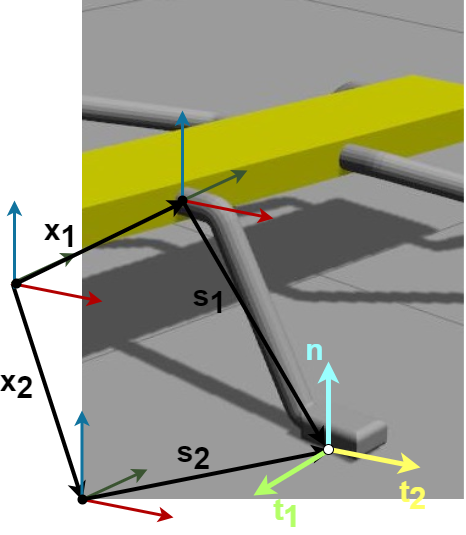
\includegraphics[height=4cm,width=1\textwidth,keepaspectratio]{Strirus_leg.drawio.png}
            \end{figure}
            \vspace{-1cm}
            \begin{align}
                \left\{\begin{matrix*}[l]
                           \mu f_n \geqslant \sqrt{f_1^2 + f_2^2}\\
                           \left\lVert \vec{v_t}\right\rVert (\mu f_n - \sqrt{f_1^2 + f_2^2}) = 0\\
                           \dfrac{\vec{f_t}}{\left\lVert \vec{f_t}\right\rVert } = - \dfrac{\vec{v_t}}{\left\lVert \vec{v_t}\right\rVert }
                       \end{matrix*}\right.
            \end{align}
        \end{column}
    \end{columns}
\end{frame}

\note{\small \setlength{\parindent}{20pt}
\begin{itemize}
    \item Для шагающих роботов критично важно правильно описать взаимодействие с опорной поверхностью. Используется модель сухого трения, описанная конусом трения.
    \item формулы 9 - функция связи для определения контакта
    \item 11 описание конуса трения
\end{itemize}


}

\begin{frame}[t]{Целевая функция}
    \framesubtitle{}
    \begin{eqnarray}
        F \rightarrow max = \beta \left( {\omega}_{1} \cdot \delta + {\omega}_{2} \cdot L\right) + (1 - \beta) {\delta}^{{\omega}_{1}} {\left( L\right)}^{{\omega}_{2}} \\
        L = \frac{1}{(\gamma - 1) h_{\text{leg}}sin(\alpha)}
    \end{eqnarray}
    \begin{columns}[T,onlytextwidth]
        \begin{column}{0.48\textwidth}
            Где
            $\beta$ -- адаптивный параметр, \\ 
            ${\omega}_{1,2} \in  [ 0..1 ],\ \omega_1 + \omega_2 = 1 $ -- весовые коэффициенты, \\
            $\delta$ -- пройденный путь, \\
            $L$ -- упрощенная длина робота

            % \textit{Для решения однокритериальной задачи} использовалась аддитивно-мультипликативная свертка
        \end{column}
        \begin{column}{0.50\textwidth}
            \begin{figure}[H]
                \centering
                \centering\includegraphics[height=3cm,width=1\textwidth,keepaspectratio,page=3]{./tikz_pictures.pdf}
                \caption*{Геометрическое представление особи}
            \end{figure}
        \end{column}
    \end{columns}
\end{frame}

\note{\small \setlength{\parindent}{20pt}
\begin{itemize}
    \item На слайде 15 формализована постановка целевой функции 
    \item В формуле дельта это пройденный путь, а L --- упрощенная длина робота, без лишних констант. Омеги --- весовые коэффициенты, их можно воспринимать следующим образом. Сумма коэффициентов равна 1. Настраивая данные коэффициенты можно показать, что в конкретной оптимизации важнее: проходимость или размеры робота.
\end{itemize}
}

\begin{frame}[t]{Закономерность}
    \begin{columns}[T,onlytextwidth]
        \begin{column}{0.49\textwidth}
            Лучшие роботы в экспериментах начинались с 10 до 14 ног для различных значений $\omega$.

            Это объясняется критерием статического равновесия. В таком случае минимум 4 ноги всегда касаются поверхности.
        \end{column}
        \begin{column}{0.49\textwidth}
            \begin{figure}[H]
                \centering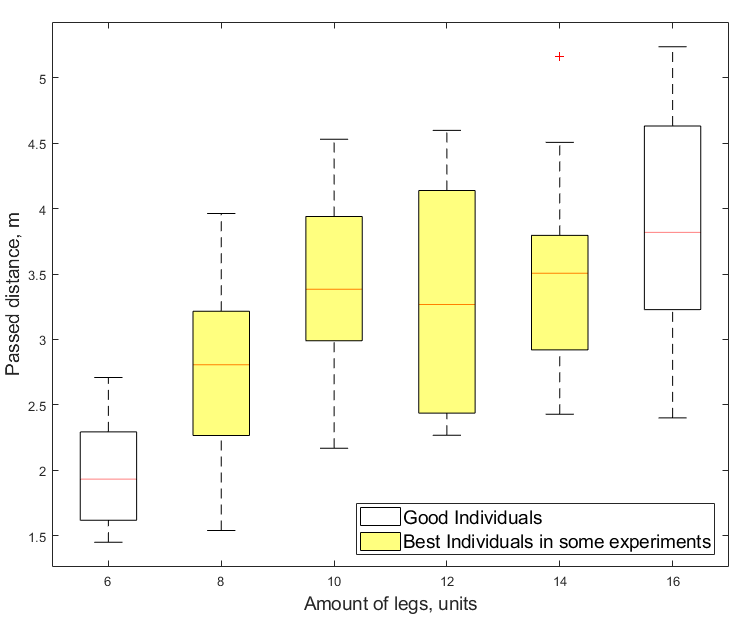
\includegraphics[height=5cm,width=1\textwidth,keepaspectratio]{box_plot_structural_synthesis.png}
                \caption*{Зависимость между кол-вом ног и пройденной дистанцией}
            \end{figure}
        \end{column}
    \end{columns}
\end{frame}

\note{\small \setlength{\parindent}{20pt}

Результатом оптимизации получена зависимость количества ног робота в зависимости от различных весов. пары омега тоже менялись. Этот массив данных собирался и был представлен в виде \textbf{блочной диаграммы с ограничителями выбросов}, где *тык* показаны квартили каждой выборки.

Лучшие результаты были получены, когда ног было от 10, до 14и.}

\begin{frame}[c]{Прототипы робота}
    \begin{figure}[H]
        \begin{subfigure}{0.32\textwidth}
            \centering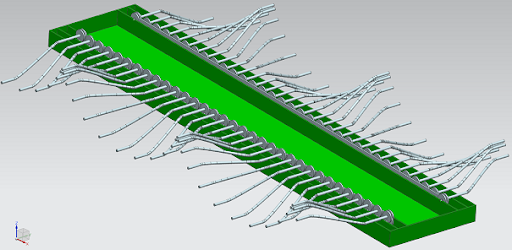
\includegraphics[height=3cm,width=1\textwidth,keepaspectratio]{strirus_0.png}
        \end{subfigure}
        \begin{subfigure}{0.32\textwidth}
            \centering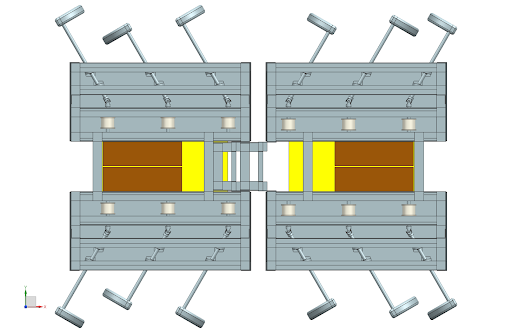
\includegraphics[height=3cm,width=1\textwidth,keepaspectratio]{strirus_1.png}
        \end{subfigure}
        \begin{subfigure}{0.32\textwidth}
            \centering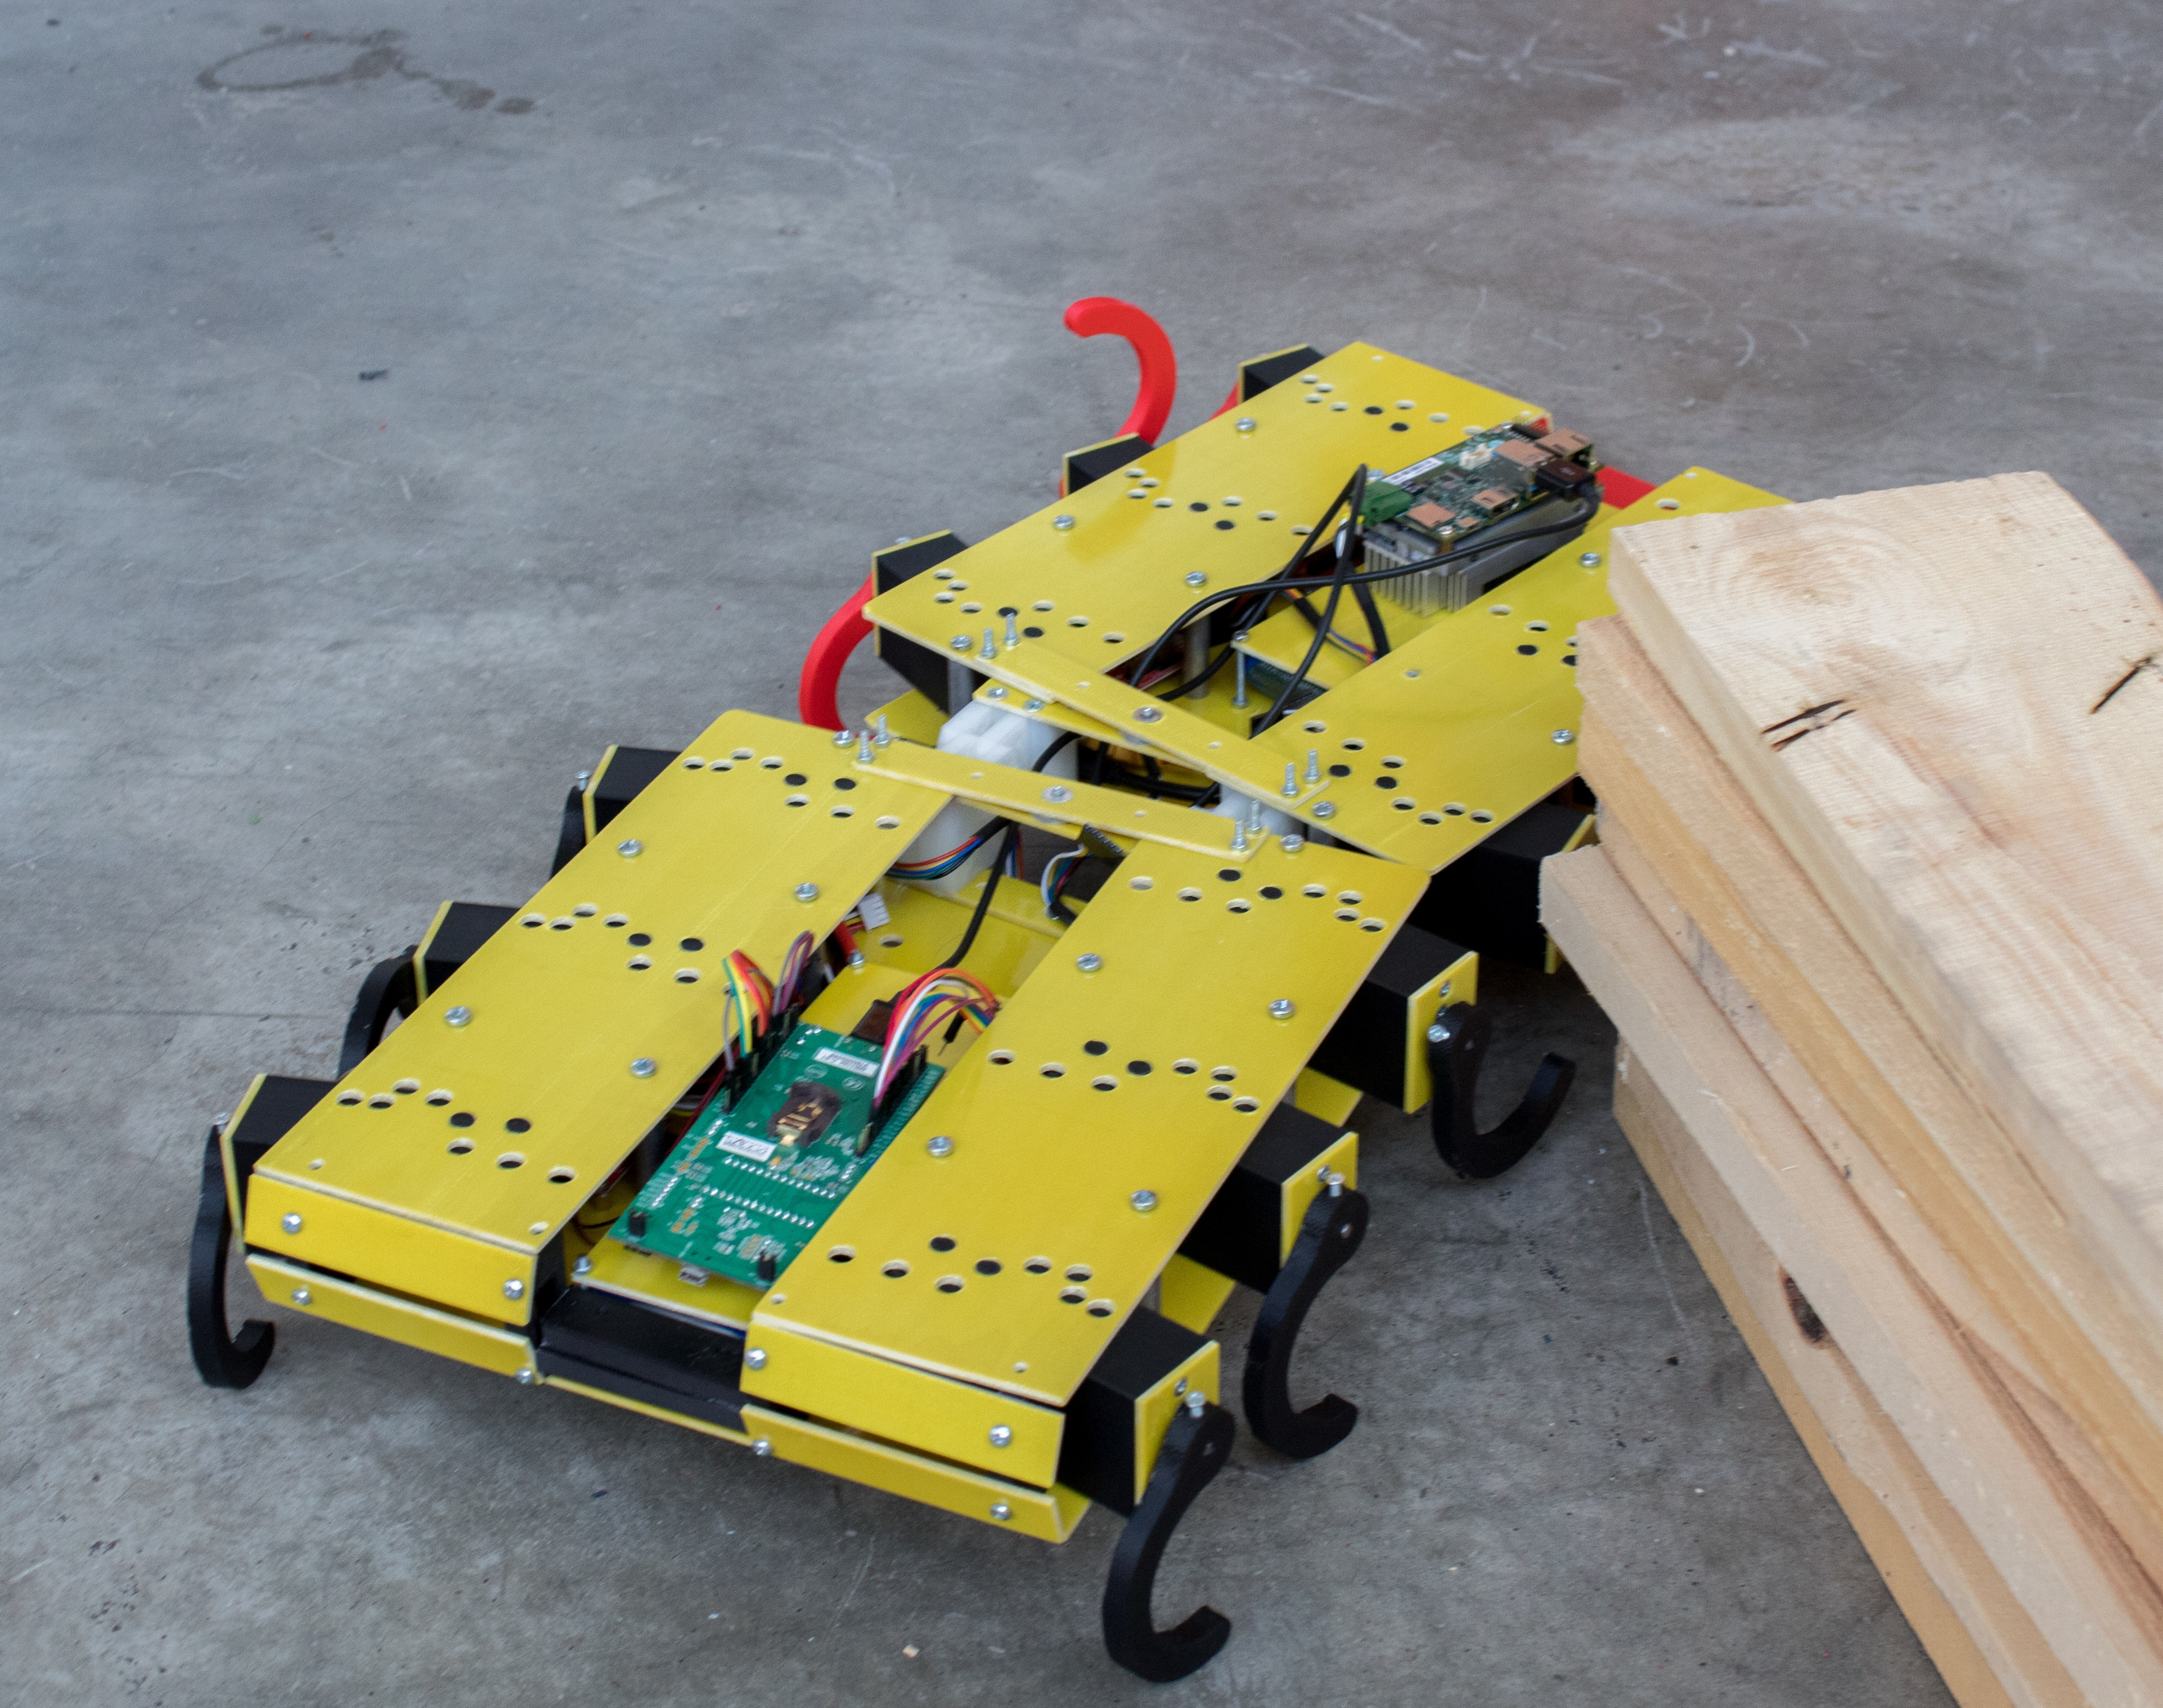
\includegraphics[height=3cm,width=1\textwidth,keepaspectratio]{strirus_2.jpg}
        \end{subfigure}

        \begin{subfigure}{0.32\textwidth}
            \centering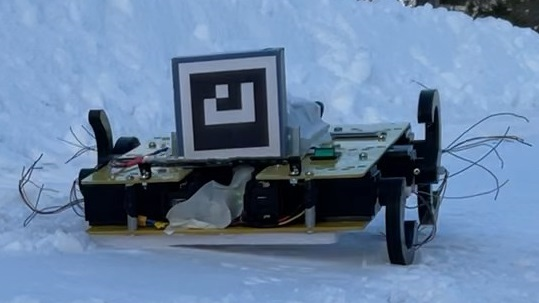
\includegraphics[height=3cm,width=1\textwidth,keepaspectratio]{strirus_3_snow.jpg}
        \end{subfigure}
        \begin{subfigure}{0.32\textwidth}
            \centering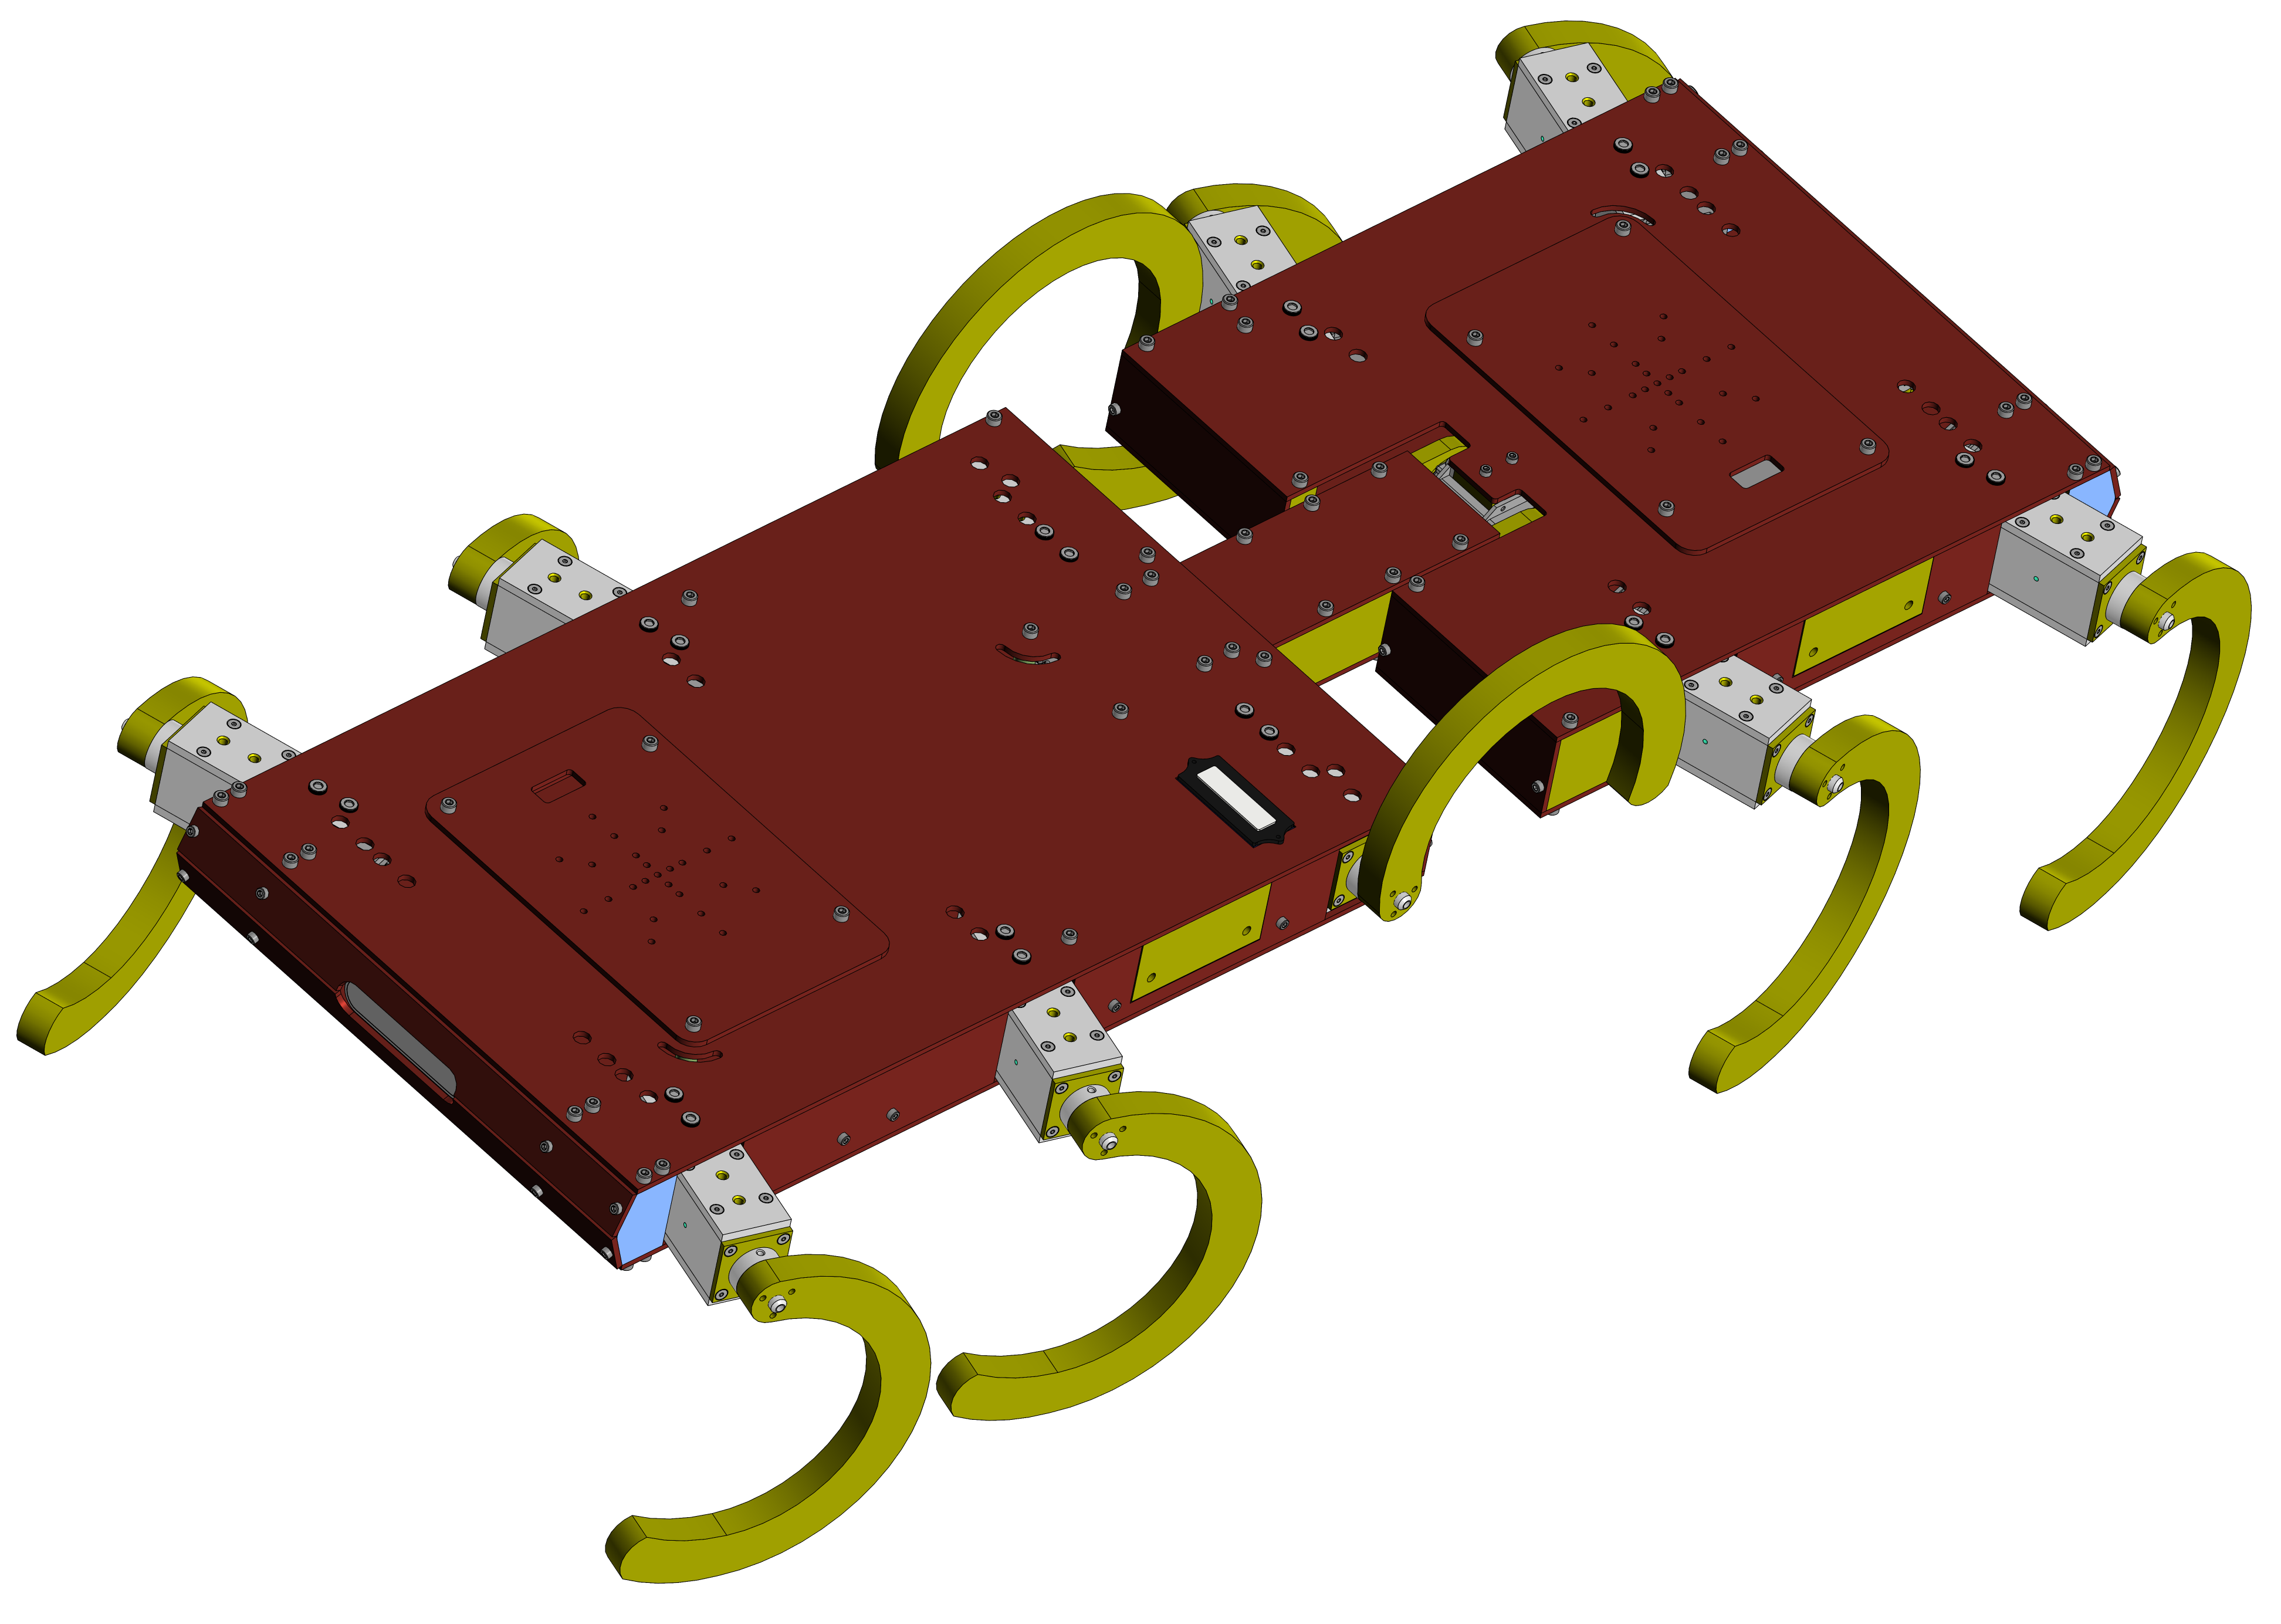
\includegraphics[height=3cm,width=1\textwidth,keepaspectratio]{strirus_4.png}
        \end{subfigure}
    \end{figure}
\end{frame}

\note{\small \setlength{\parindent}{20pt}
\begin{itemize}
    \item На основе полученной зависимости, разрабатывались различные прототипы. Можно выделить 5 прототипов, 2 из которых были собраны натурно. Более того, один был апробирован в приближенных к реальным условиях среде, в снегу *тык*.
    \item Были роботы с одним и без сочленений, менялась длина ног.
    \item Экспериментально было выяснено, что 10 ног лучше, чем 12, так как при той же длине корпуса, можно сильно увеличить длину ног, что сильно влияет на профильную проходимость.
\end{itemize}
}

\begin{frame}[c]{Особенности конструкции}
    \framesubtitle{}
    \begin{figure}[H]
        \begin{subfigure}{0.39\textwidth}
            \centering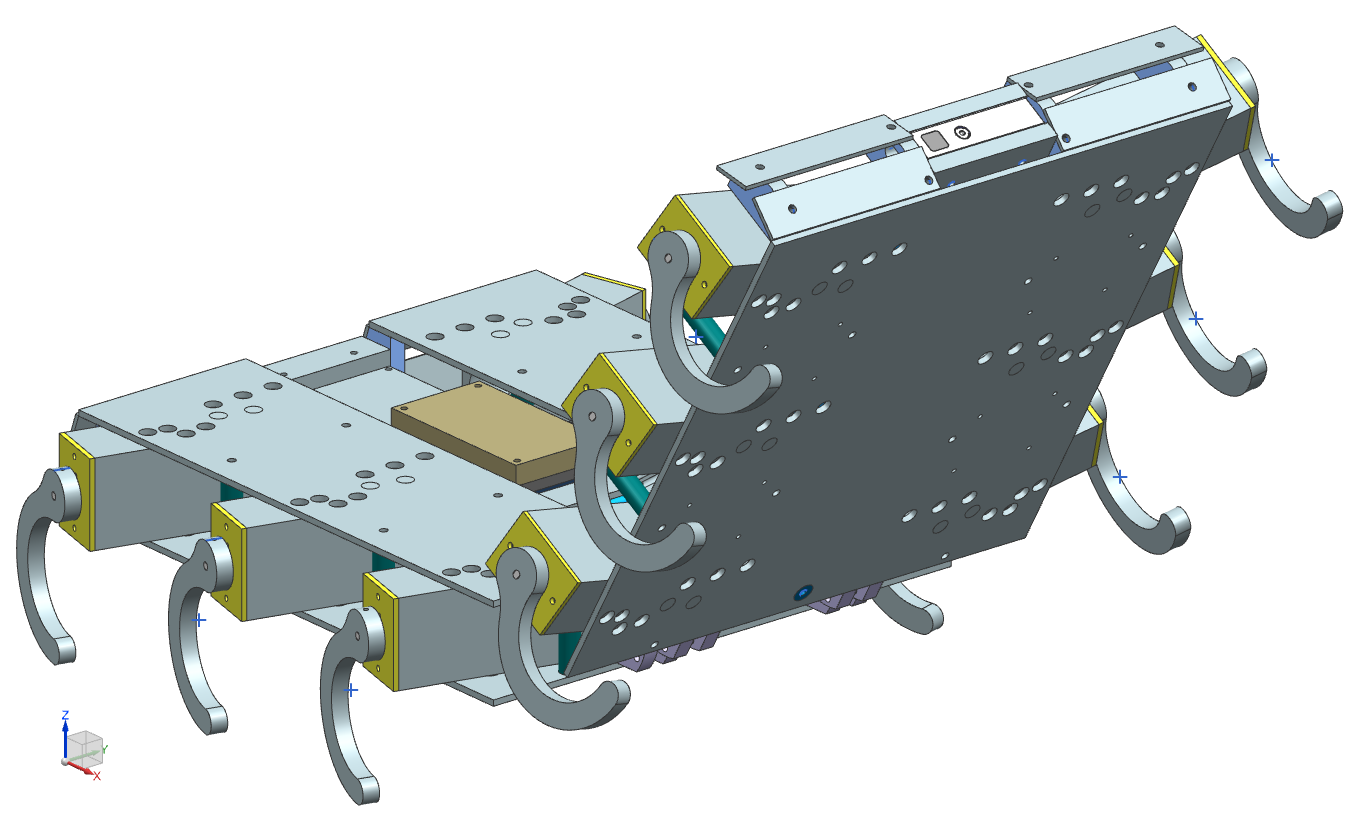
\includegraphics[height=6cm,width=1\textwidth,keepaspectratio]{17.png}
            \caption*{Одностепенной активный сегмент, соединяющий 2 части робота}
        \end{subfigure}
        \begin{subfigure}{0.59\textwidth}
            \centering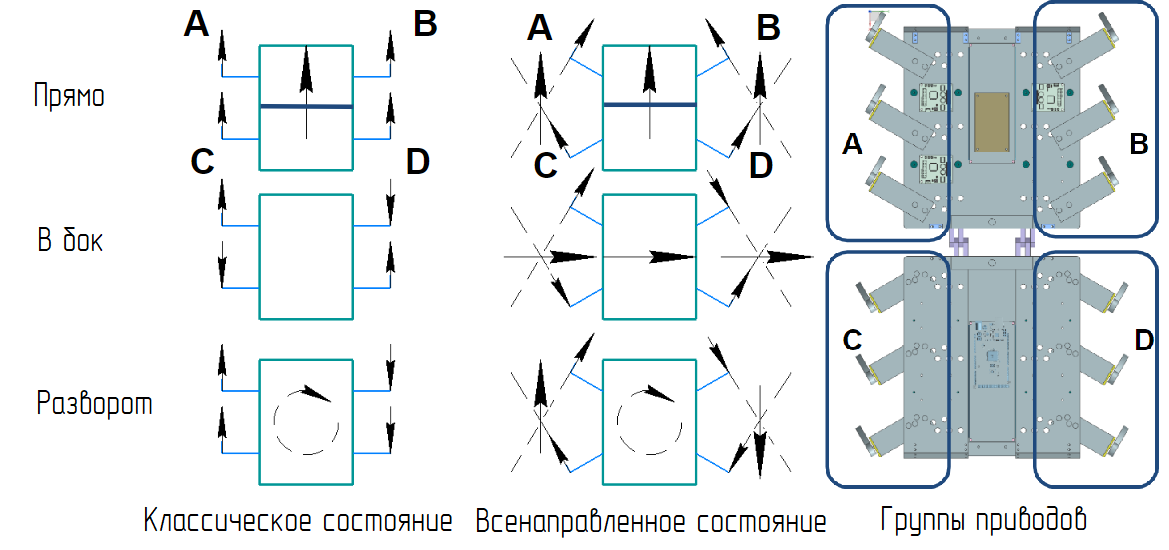
\includegraphics[height=6cm,width=1\textwidth,keepaspectratio]{vector_representation_rus}
            \caption*{Векторное представление сил в обычном и всенаправленном состояниях}
        \end{subfigure}
    \end{figure}
\end{frame}

\note{\small \setlength{\parindent}{20pt}
\begin{itemize}
    \item Особенности последнего прототипа в следующем. Во первых, был добавлен активный сегмент, соединяющий 2 части робота *тык*. Это позволяет добиться условия, чтобы робот мог забраться на препятствия выше себя ростом. 
    \item Также, была придуман концепт, позволяющий двигаться такому классу роботов без смены ориентации во все стороны. Я вдохновлялся омниколесом
\end{itemize}
}

\begin{frame}[t]{Четвертая итерация робота}
    \framesubtitle{}
    \begin{figure}[H]
        \centering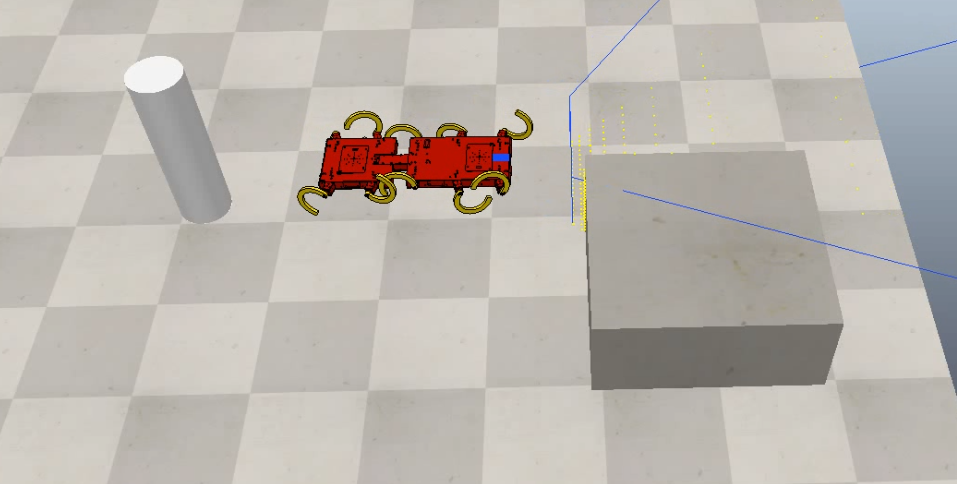
\includegraphics[height=6cm,width=1\textwidth,keepaspectratio]{sidestep_segment_video_preview.png}
    \end{figure}
\end{frame}

\note{\small \setlength{\parindent}{20pt}

На видео представлено прохождение препятствий последним прототипом робота в симуляторе CoppeliaSim}
\section{"4" Верификация преобразователя силы}

\begin{frame}[t]{Верификация преобразователя силы}
\framesubtitle{}
\begin{columns}[T,onlytextwidth]
\begin{column}{0.69\textwidth}
    \small
    \underline{Измерить характеристики} материала для случаев, когда \textbf{площадь приложения силы меньше}, чем \textbf{площадь активной части} сенсора.

    \textbf{Алгоритм}: 2 эксперимента: 
    
    1. Статический --- прикладывается статический груз с размером в сенсор для \underline{калибровки}.\\
    2. Динамический --- чувствительная область представляется в виде сетки $4\times4$. Происходит \textbf{касание} каждой \underline{области} \textbf{c одинаковым давлением}, но \underline{разной площадью контакта}.

    \textbf{Входные данные}: показания разработанного датчика и значение реально приложенной нагрузки.

    \textbf{Выходные данные}: разница между нормализованным значением с датчика и реальной нагрузкой.

    \textbf{Допустимая ошибка}: 10\%

    \textbf{Предположения}: 1) материал обладает вязко-эластичными свойствами, поэтому надо учитывать гистерезис.
\end{column}
\begin{column}{0.29\textwidth}
    \vspace{-1.0cm}
\begin{figure}[H]
\begin{subfigure}{0.99\textwidth}
        \centering
        \centering\includegraphics[height=3cm,width=1\textwidth,keepaspectratio,page=5]{./tikz_pictures.pdf}
        \caption*{Поверхность \\ как $4\times4$ сетка}
\end{subfigure}

\begin{subfigure}{0.99\textwidth}
    \centering\includegraphics[height=3cm,width=1\textwidth,keepaspectratio,page=4]{./tikz_pictures.pdf}
    \caption*{Все насадки}
\end{subfigure}

\end{figure}
\end{column}
\end{columns}
\end{frame}

\note{\small \setlength{\parindent}{20pt}

Решив задачу номер 3, то есть имея конструкцию ноги, возможно разработать сенсор, подходящий для конкретной области применения. Как было сказано ранее, необходимо измерить характеристики материала для случаев когда площадь приложения силы меньше, чем площадь активной части сенсора.

Для этого было разработано 2 эксперимента. Первый, статический, где на объект прикладывался статический груз с размером сенсора, нужен для калибровки. Таким образом я считал, что все сенсоры работают единообразно.

Второй, динамический, основной. Для этого сенсор представлялся в виде сетки 4х4, на картинке *тык*. С помощью эталонного датчика силы, на который была прикреплена насадка *тык*, обеспечивающую конкретную площадь контакта, проводилась касание каждой области сетки. 

После эксперимента, нормализовались значения между эталонным датчиком (его значения принимались за 1), и откалиброванным исследуемым датчиком. Смотрелась разница. 

Допустимой ошибкой я посчитал 10 процентов, такая ошибка принята в физических экспериментах.
}

\begin{frame}[t]{Статический эксперимент}
    \begin{columns}[T,onlytextwidth]
        \begin{column}{0.52\textwidth}
            \begin{eqnarray}
                V_{out} = V_0 + p[k_p + k_e(1-e^\frac{-(t-t_0)}{\tau_{res}})](1-e^{-\frac{A}{p}}) \\
                k_p = A_1e^{-A_2p} \\ \tau_{res} = B_0 + B_1e^{-\frac{p}{B_2}}
            \end{eqnarray}
            Где $V_0$ -- начальное напряжение, \\ $p$ -- приложенное давление, \\ $A_i,\ B_i,\ \tau_{res},\ k_i$ искомые параметры, \\  $t$ -- текущее время, $t_0$ -- время начала нажатия.
            % \\ \alert{Апробированна модель для калибровки датчика}
        \end{column}
        \begin{column}{0.45\textwidth}
            \vspace{-0.5cm}
            \begin{figure}[H]
                \begin{subfigure}{0.99\textwidth}
                    \centering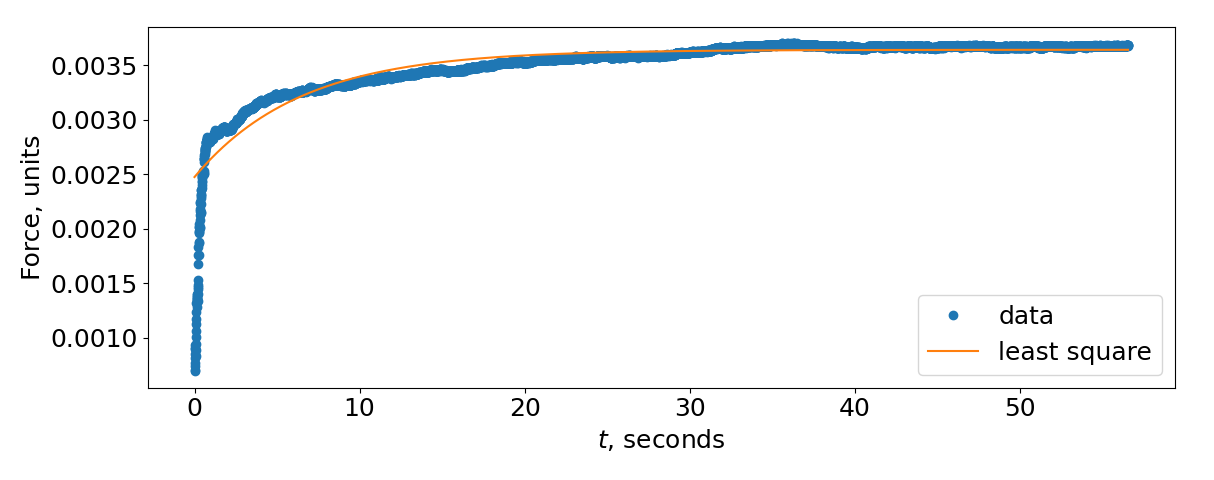
\includegraphics[height=2.8cm,width=1\textwidth,keepaspectratio]{least_square_model.png}
                    \caption*{График регрессии}
                \end{subfigure}

                \vspace{-0.3cm}
                \begin{subfigure}{0.99\textwidth}
                    \centering
                    \centering\includegraphics[height=3.4cm,width=1\textwidth,keepaspectratio,page=6]{./tikz_pictures.pdf}
                    \caption*{Экспериментальная установка}
                \end{subfigure}
            \end{figure}
        \end{column}
    \end{columns}
\end{frame}

\note{\small \setlength{\parindent}{20pt}

Статический эксперимент. Для калибровки использовался робастный метод наименьших квадратов, экспериментальная установка справа *тык*, формула для регрессии --- слева *тык*. Она основана на знании того, что у нас вязко-эластичный материал, обладающий гистерезисом. Поэтому необходимо учитывать время контакта с поверхностью.

Экспериментальная установка показана ниже *тык*.

Как можно заметить по графику справа, эта формула подходит для калибровки.}

\begin{frame}[t]{Динамический эксперимент: Установка}
    \vspace{0.2cm}
    \centering\includegraphics[height=6.5cm,width=1\textwidth,keepaspectratio,page=7]{./tikz_pictures.pdf}
\end{frame}

\note{\small \setlength{\parindent}{20pt}

Так как динамический эксперимент требует многократное повторение действий, где важна точность силы нажатия, то было решено создать автоматизированную робототехническую установку *тык*. 

Минимизация ошибки по установке манипулятора была реализована с помощью технического зрения.

Манипулятор необходим, так данная установка позволяет проводить не только контактные эксперименты, но также и прокатывать вали по сенсору, что ближе к кинематике движения робота. Более того, мы можем проверять и калибровать сенсор уже установленный на ногу робота.
}

\begin{frame}[t]{Результаты динамического эксперимента}
    \begin{figure}[H]
        \begin{subfigure}{0.49\textwidth}
            \centering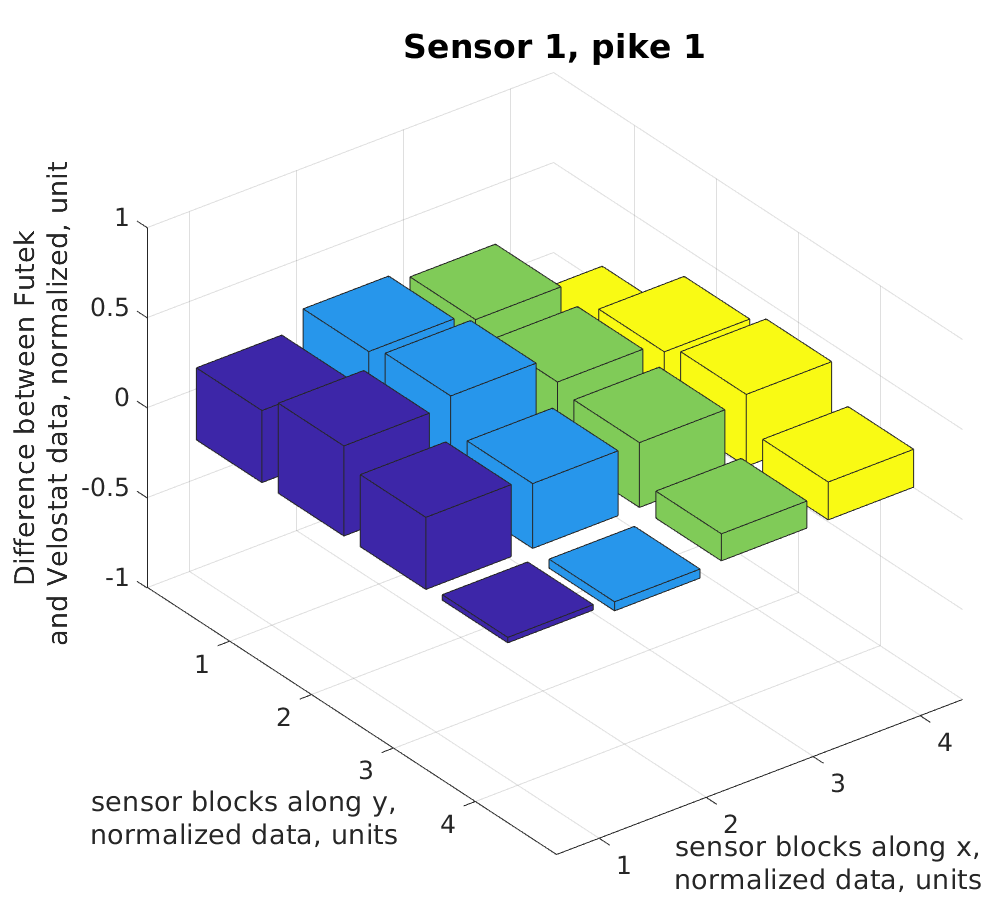
\includegraphics[height=5cm,width=1\textwidth,keepaspectratio]{sens1_pike1.png}
            \caption*{2 мм диаметр насадки}
        \end{subfigure}
        \begin{subfigure}{0.49\textwidth}
            \centering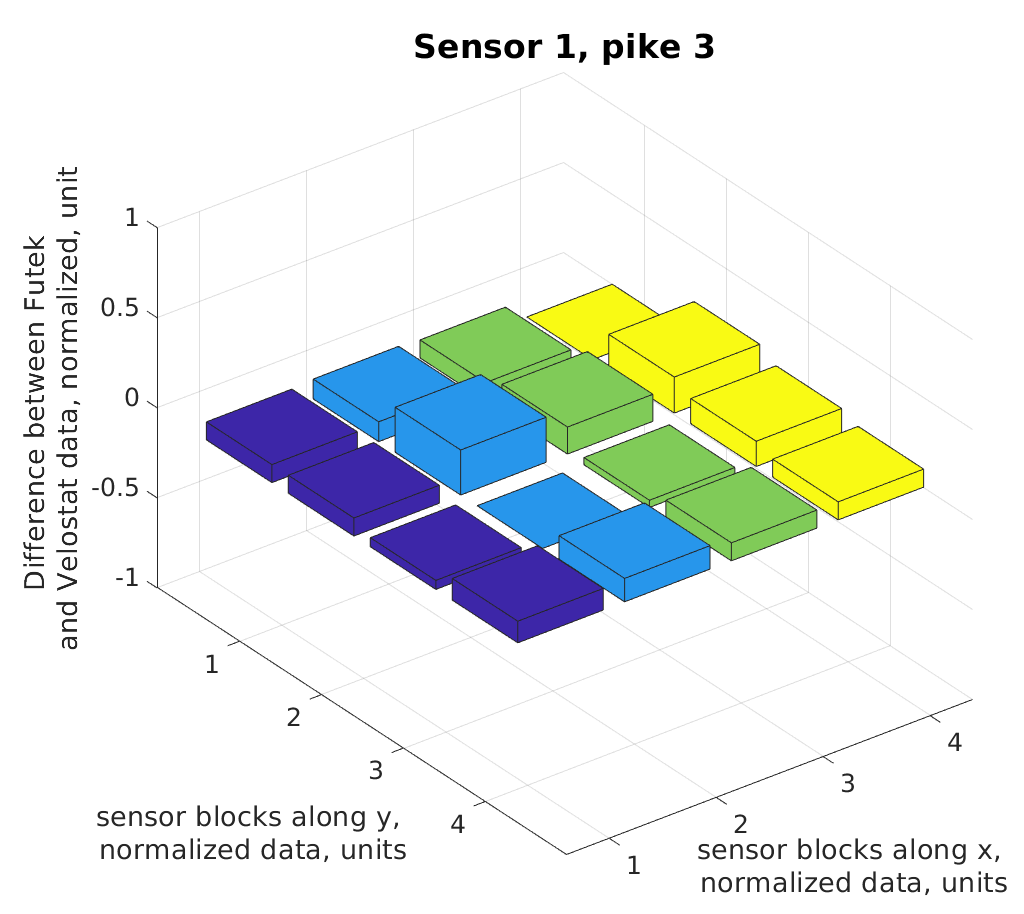
\includegraphics[height=5cm,width=1\textwidth,keepaspectratio]{sens1_pike3.png}
            \caption*{8 мм диаметр насадки}
        \end{subfigure}
    \end{figure}
    \vspace{-0.8cm}
    \alert{Одинаковые данные, когда площадь нажатия превышает 25\% от площади датчика}
\end{frame}

\note{\small \setlength{\parindent}{20pt}

Результатом изысканий получилось, что можно использовать сенсор, когда площадь нажатия превышает 25 площади датчика.

На слайде можно увидеть 3д гистограмму *тык*, где представлена нормализованная разница между эталонным датчиком и исследуемым для каждого сегмента датчика. Слева при использования насадки в 2 мм диаметром, а справа при 8 мм.
}
\section{"3" Определение физико-механических свойств поверхности}

\begin{frame}[t]{"3" Определение физико-механических свойств}
    \framesubtitle{}
    \small
    Определить процентное соотношение твердых, упругих и пластичных свойств пройденной поверхности

    \textbf{Метод решения}: машинное обучение, Метод Опорных Векторов (SVM)

    \textbf{Алгоритм}: Создается \underline{установка} для обучения. \underline{Обучение}: робот ходит по различным типам поверхностей фиксированное количество касаний поверхности с постоянной угловой скоростью. Модель обучается на 80\% данных с помощью ядра PUK7. \underline{Тестирование}: происходит на оставшихся 20\%.  Используются \textbf{метрики} меткости, точности, полноты и F1-счета.

    \begin{columns}[T,onlytextwidth]
        \begin{column}{0.44\textwidth}
            \textbf{Входные данные}: данные с внутренних датчиков робота

            \textbf{Выходные данные}: процентное соотношение упругих, твердых и пластичных свойств пройденной поверхности

            \textbf{Допустимая ошибка}: 20\% - точность

            \textbf{Предположения}: 1) На рисунке.

        \end{column}
        \begin{column}{0.54\textwidth}
            
            \vspace{-0.5cm}
            \begin{table}[H]
                \centering
                \resizebox{\linewidth}{!}{%
                \begin{tblr}{
                    row{2} = {c},
                    row{3} = {c},
                    cell{1}{2} = {c},
                    cell{1}{3} = {c},
                    cell{1}{4} = {c},
                    % vline{2} = {2-3}{},
                    % hline{2} = {2-4}{},
                }
                 & \textbf{Упругая} & \textbf{Твердая} & \textbf{Пластичная}\\
                \begin{sideways}\textbf{Пещера}\end{sideways} & \centering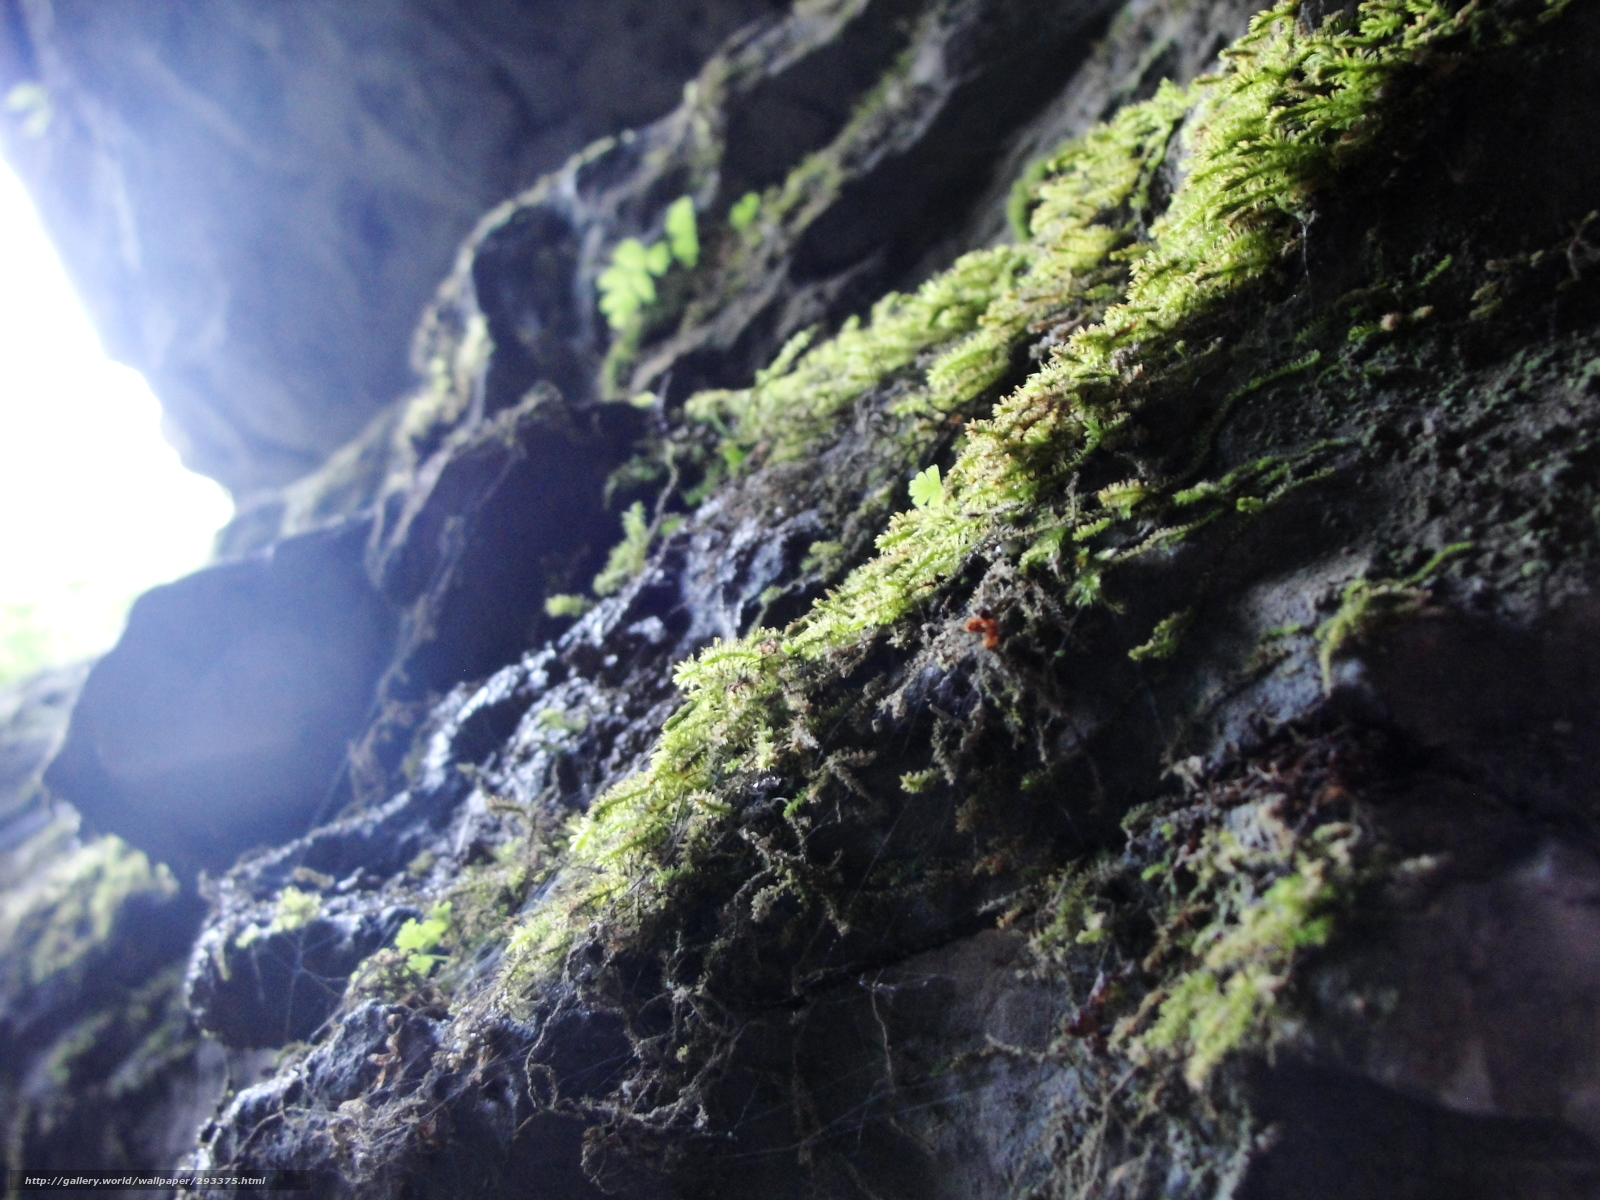
\includegraphics[height=1.5cm,width=1\textwidth,keepaspectratio]{surface_types/moss.jpg} & \centering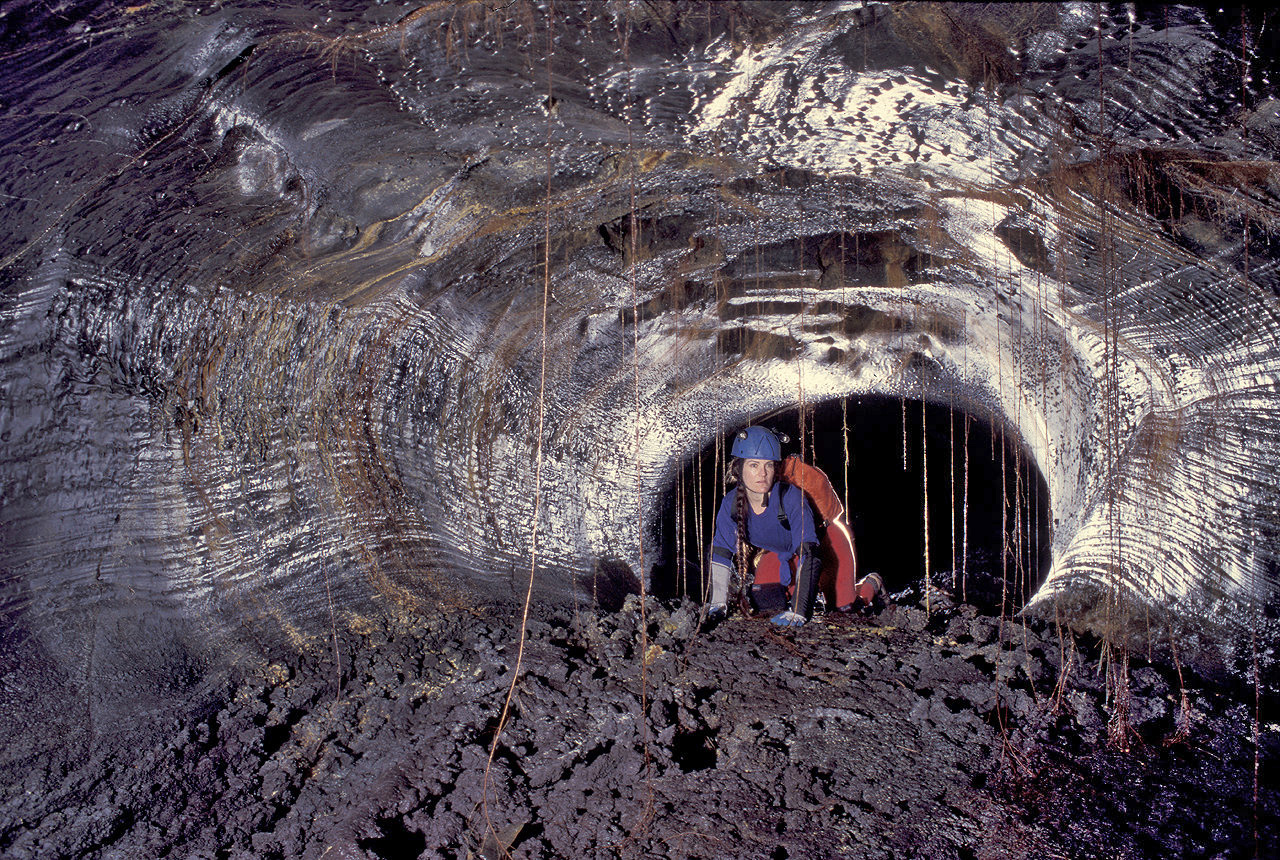
\includegraphics[height=1.5cm,width=1\textwidth,keepaspectratio]{surface_types/lava.jpg} & \centering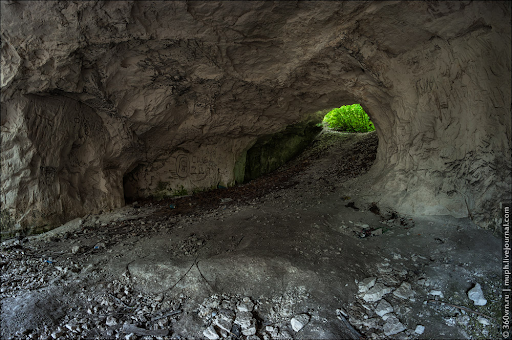
\includegraphics[height=1.5cm,width=1\textwidth,keepaspectratio]{surface_types/moul.png}\\
                \begin{sideways}\textbf{Установка}\end{sideways} & \centering\includegraphics[height=1.5cm,width=1\textwidth,keepaspectratio]{surface_types/rubber.JPG} & \centering\includegraphics[height=1.5cm,width=1\textwidth,keepaspectratio]{surface_types/rock.jpg} & \centering\includegraphics[height=1.5cm,width=1\textwidth,keepaspectratio]{surface_types/zemlya.jpg}
                \end{tblr}
                }
                \end{table}
            % \begin{figure}[H]
            %     \begin{subfigure}[b]{0.3\textwidth}
            %         \centering\includegraphics[height=1.5cm,width=1\textwidth,keepaspectratio]{surface_types/moss.jpg}
            %     \end{subfigure}
            %     \hfill
            %     \begin{subfigure}[b]{0.3\textwidth}
            %         \centering\includegraphics[height=1.5cm,width=1\textwidth,keepaspectratio]{surface_types/lava.jpg}
            %     \end{subfigure}
            %     \hfill
            %     \begin{subfigure}[b]{0.3\textwidth}
            %         \centering\includegraphics[height=1.5cm,width=1\textwidth,keepaspectratio]{surface_types/moul.png}
            %     \end{subfigure}

            %     \begin{subfigure}[b]{0.3\textwidth}
            %         \centering\includegraphics[height=1.5cm,width=1\textwidth,keepaspectratio]{surface_types/rubber.JPG}
            %     \end{subfigure}
            %     \hfill
            %     \begin{subfigure}[b]{0.3\textwidth}
            %         \centering\includegraphics[height=1.5cm,width=1\textwidth,keepaspectratio]{surface_types/rock.jpg}
            %     \end{subfigure}
            %     \hfill
            %     \begin{subfigure}[b]{0.3\textwidth}
            %         \centering\includegraphics[height=1.5cm,width=1\textwidth,keepaspectratio]{surface_types/zemlya.jpg}\\
            %     \end{subfigure}
            %     \vspace{-0.3cm}
            %     \caption{Эталоны упругой, твердой и пластичной поверхностей}
            % \end{figure}
        \end{column}
    \end{columns}
\end{frame}

\note{\small \setlength{\parindent}{20pt}

Решив задачи 3 и 4, то есть имея разработанный сенсор и узел с ногой робота, возможно решать задачу определения физико-механических свойств поверхности. Для получения более точных результатов, было решено решать данную задачу натурно.

Любой материал можно описать с помощью вязко-упруго-пластичной модели, но их сложно померить и еще сложнее интерпретировать. Поэтому более целесообразно классифицировать объекты, которые использовались как эталонно упругие, твердые и пластичные *тык*. Аналогом мха --- эталона упругих свойств является резина, твердой --- камень, а пластичной --- земля. Результатом работы алгоритма получается процентное соотношение  упругих, твердых и пластичных свойств.

Для решения задачи классификации используется метод опорных векторов (SVM). Данные собирались так. Робот ходит по различным типам поверхностей фиксированное количество касаний поверхности с постоянной угловой скоростью. Данные с внутренних датчиков, о которых будет разговор далее, собираются. Потом происходит обучение и тестирование. Использовались классические критерии для данного типа задачи: меткость, точность, полнота и F1-счет. Это классические метрики оценки точности обученной модели.
}

\begin{frame}[t]{Стенд}
    \framesubtitle{}
    \begin{figure}[H]
        \begin{subfigure}[t]{0.33\textwidth}
            \centering\includegraphics[height=5cm,width=1\textwidth,keepaspectratio]{s_shape_leg/rockk.png}
            \caption*{Установка}
        \end{subfigure}
        \begin{subfigure}[t]{0.33\textwidth}
            \centering\includegraphics[height=5cm,width=1\textwidth,keepaspectratio]{s_shape_leg/socks.jpg}
            \caption*{Нога робота с установленными сенсорами}
        \end{subfigure}
        \begin{subfigure}[t]{0.33\textwidth}
            \centering\includegraphics[height=5cm,width=1\textwidth,keepaspectratio]{s_shape_leg/leg_design.png}
            \caption*{Схематическое распределение сенсоров на ноге}
        \end{subfigure}
    \end{figure}
\end{frame}

\note{\small \setlength{\parindent}{20pt}

На экране представлен стенд *тык*, нога робота, на которую установлены датчики силы *тык*, а также способ установки сенсоров на ногу *тык*. 

Нужно отметить, что во время испытаний, пришел к выводу, что максимум нужно 5 сенсоров, а не 8, как указано на рисунке справа.

На видео показана работа стенда во время обучения.
}

\begin{frame}[t]{Метод опорных векторов}
    \framesubtitle{}
    \small

    \begin{columns}[T,onlytextwidth]
        \begin{column}{0.49\textwidth}
            \vspace{-0.5cm}
            \begin{align}
                f(x) = w^T x + b
            \end{align}

            \vspace{-0.2cm}

            где $w$ --- весовой вектор, $b$ --- смещение,

            $x$ --- \textbf{входной вектор}:

            (1) Частота движения ног\\
            (2-12) Данные с датчика силы\\
            (13-16) Данные крутящего момента двигателя\\
        \end{column}
        \begin{column}{0.49\textwidth}
            Ядро на основе функции Пирсона VII:
            \begin{align}
                K(x, y) = (1 + ((||x - y||^2)/\sigma^2)^\omega)^{(-1/\omega)}
            \end{align}

            \vspace{-0.2cm}

            Где $x$, $y$ --- векторы во входном пространстве, $||x - y|||$ --- евклидово расстояние между $x$ и $y$, $\sigma$ --- масштабный параметр; $\omega$ --- это параметр формы.
        \end{column}
    \end{columns}
    \vspace{-0.4cm}
    \begin{figure}[H]
        \begin{subfigure}[t]{0.49\textwidth}
            \centering\includegraphics[height=3cm,width=1\textwidth,keepaspectratio]{../images/s_shape_leg/avg_lin_vel_rev_min.png}
            \caption*{Зависимость угловой скорости от линейного перемещения}
        \end{subfigure}
        \begin{subfigure}[t]{0.49\textwidth}
            \centering\includegraphics[height=3cm,width=1\textwidth,keepaspectratio]{../images/s_shape_leg/TaxelIndForce.png}
            \caption*{Распределение силы нажатия на каждый сенсор}
        \end{subfigure}
    \end{figure}
\end{frame}

\note{\small \setlength{\parindent}{20pt}

Метод опорных векторов --- алгоритм обучения с учителем. описывается следующей формулой *тык*. Главная цель SVM как классификатора --- найти уравнение разделяющей гиперплоскости. 

Входной вектор включал в себя частоту движения ног *тык*, так как показано на рисунке справа - он может критерием определения, так как при одинаковой частоте вращения, линейное перемещение разное. 

Информация с датчиков силы *тык*. На графиках одно нажатие ноги на резину, камень и землю. На оси х --- время, на оси ординат --- сила на каждом конкретном датчике силы. Как видно, разный характер распределения сил в зависимости от материала. также с мотора - основные показания.

Также снимались данные о моменте с мотора.

Так как у нас задача нелинейная, то использовался kernel trick. Функция ядра обычно преобразует обучающий набор данных таким образом, что нелинейная поверхность принятия решений способна преобразовываться в линейное уравнение в пространствах большего числа измерений. Для этого использовалась функция Пирсона VII.
}

\begin{frame}[t]{Результаты}
    \framesubtitle{}
    \begin{columns}[T,onlytextwidth]
        \begin{column}{0.49\textwidth}
            \begin{table}[H]
                \resizebox{\linewidth}{!}{%
                    \begin{tabular}{|c|c|c|c|c|}
                        \cline{3-5}
                        \multicolumn{1}{l}{}                     & \multicolumn{1}{l|}{} & \multicolumn{3}{c|}{\textbf{Предсказанный класс}}                                                                                           \\
                        \cline{3-5}
                        \multicolumn{1}{l}{}                     &                       & Камень                                            & Резина                                     & Земля                                      \\
                        \hline
                        \multirow{3}{*}{{\textbf{Истин. класс}}} & Камень                & {\cellcolor[rgb]{0.741,0.843,0.929}}84.0\%        & 2.56\%                                     & 13.44\%                                    \\
                        \hhline{|~----|}
                                                                 & Резина                & 20.1\%                                            & {\cellcolor[rgb]{0.741,0.843,0.929}}67.8\% & 12.1\%                                     \\
                        \hhline{|~----|}
                                                                 & Земля                 & 1.0\%                                             & 18.9\%                                     & {\cellcolor[rgb]{0.741,0.843,0.929}}80.1\% \\
                        \hline
                    \end{tabular}
                }
                \caption{Результаты обученного классификатора опорных поверхностей}
            \end{table}

            Камень --- эталон твердых свойств поверхности;\\
            Резина --- эталон упругих свойств;\\
            Земля --- эталон пластичных свойств.
        \end{column}
        \begin{column}{0.49\textwidth}
            \begin{figure}[H]
                \centering\includegraphics[height=5cm,width=1\textwidth,keepaspectratio]{../images/s_shape_leg/feature_score.png}
                \caption*{Гистограмма влияния входных данных на результат предсказания}
            \end{figure}
        \end{column}
    \end{columns}
\end{frame}

\note{\small \setlength{\parindent}{20pt}

На слайде представлены результаты классификации опорных поверхностей *тык*. 

Ее можно интерпретировать следующим образом. В камне 84 процента твердых свойств, 2.5 упругих и 13.44 пластичных. В резине --- 20 процентов твердых, 67.8 упругих и 12.1 --- пластичных.

Не менее важный вопрос, какие данные оказали самый весомый вклад в определении физико-механических свойств. Для этого была построенная гистограмма влияния входных данных *тык*.

Верхний график --- когда брались все данные, нижний --- без показаний с мотора.

На основе гистограммы можно увидеть, что момент на моторе и частота вращения имеют большее влияние на предсказание, чем данные о силе нажатия.
}
\section{"4" Определение геометрических свойств поверхности}

\begin{frame}[t]{"4" Определение геометрических свойств}
\framesubtitle{}
    \begin{columns}[T,onlytextwidth]
        \begin{column}{0.69\textwidth}
            \small
            С помощью \textbf{ощупывания роботом поверхности} получить \underline{плотное облако точек} и \underline{полигональную сетку}.

            \textbf{Метод решения}: Триангуляция Делоне с использованием альфа формы

            \textbf{Алгоритм}: Решив задачу локализации, получить облако точек следовой дорожки. \textbf{Очистить шумное облако точек} и его \textbf{усреднить} с помощью Voxel Grid. Применить \underline{триангуляцию Делоне для вогнутых оболочек}, получив полигональную сетку. \underline{Сгенерировать новые точки} из полигональной сетки с нужным разрешением.

            \textbf{Входные данные}: следовая дорожка, в виде облака точек.
            
            \textbf{Выходные данные}: полигональная сетка и плотное облако точек
            
            \textbf{Допустимая точность}: 0.1 м, оценки Cloud2Cloud и Cloud2Mesh

            \textbf{Предположения}: 1) Имеется поверхность. Координаты задаются $z=f(x,y)$. 2) Расстояние между ногами робота мало относительно размеров поверхности, следовательно, поверхность между ногами считается плоскостью.   
        \end{column}
        \begin{column}{0.29\textwidth}
            \begin{figure}[H]
                \begin{subfigure}{0.99\textwidth}
                    \centering\includegraphics[height=2.5cm,width=1\textwidth,keepaspectratio]{../images/slides/delone_mag.png}
                    \caption*{Триангуляция Делоне}
                \end{subfigure}

                \begin{subfigure}{0.99\textwidth}
                    \centering\includegraphics[height=2.5cm,width=1\textwidth,keepaspectratio]{../images/slides/error.png}
                    \caption*{Когда $z\neq f(x,y)$}
                \end{subfigure}
            \end{figure}
        \end{column}
    \end{columns}
\end{frame}

\note{\small \setlength{\parindent}{20pt}
\begin{itemize}
    \item Решив 1 и 2 задачу по определению рельефа пройденной поверхности
    \item Для получения полигональной сетки используется следовая дорожка и на разреженное облако точек применяется Делоне.
    \item Это работает из-за предположения, что расстояние между ногами робота мало относительно размеров поверхности. Поэтому эта поверхность будет считаться плоскостью
\end{itemize}
}

\begin{frame}[t]{Оценки C2C и C2M}
\framesubtitle{}
    \begin{figure}[H]
        \begin{subfigure}[t]{0.49\textwidth}
            \centering\includegraphics[height=4.5cm,width=1\textwidth,keepaspectratio]{../images/slides/c2c.png}
            \caption*{Cloud to Cloud: высчитывается абсолютное расстояние до ближайшей соседней точки}
        \end{subfigure}
        \begin{subfigure}[t]{0.49\textwidth}
            \centering\includegraphics[height=4.5cm,width=1\textwidth,keepaspectratio]{../images/slides/c2m.png}
            \caption*{Cloud to Mesh: высчитывается расстояние с учетом знания о векторе нормали плоскости}
        \end{subfigure}
    \end{figure}
\end{frame}

\note{\small \setlength{\parindent}{20pt}
\begin{itemize}
    \item Критериями оценки были выбраны 2 подхода Cloud2Cloud и Cloud2Mesh. Это стандартные метрики для сравнения облаков точек в программных продуктах.
    \item Идея в том, что С2С *тык* использует абсолютное расстояние до ближайшей соседней точки, а C2M *тык* учитывает еще в каком направлении идет отклонение от полигональной сетки.
\end{itemize}
}

\begin{frame}[t]{Эксперименты}
    \begin{figure}[H]
        \begin{subfigure}[t]{0.49\textwidth}
            \centering\includegraphics[height=5cm,width=1\textwidth,keepaspectratio]{coppelia_sim.png}
            \caption*{CoppeliaSim симулятор,\\ \textbf{4е поколение} СтриРус}
        \end{subfigure}
        \begin{subfigure}[t]{0.49\textwidth}
            \centering\includegraphics[height=5cm,width=1\textwidth,keepaspectratio]{rl_sim.JPG}
            \caption*{Натурные испытания,\\ \textbf{3е+ поколение} СтриРус}
        \end{subfigure}
    \end{figure}
\end{frame}

\note{\small \setlength{\parindent}{20pt}
\begin{itemize}
    \item Эксперименты проводились как в симуляторе, где использовался последний прототип робота, а также натурно.
    \item Эксперимент выглядел следующим образом. Генерировалось семейство поверхностей и робот ходил с помощью ручного управления определенное время. Полученное облако точек сравнивалось либо с сгенерированным, либо с измеренным в реальной жизни.
\end{itemize}


}

\begin{frame}[t]{Задача локализации}
\framesubtitle{}
\begin{align}
        H_{leg}^{glob} = H(x_{glob},y_{glob},z_{glob},\alpha_{glob},\beta_{glob},\gamma_{glob})T_z(l_1)T_x(l_2)R_y(\alpha_3)T_x(l_4)T_y(l_5)R_z(-15^{\circ})T_y(l_7)R_y(\alpha_8)
\end{align}

\vspace{-0.3cm}
Где $H = \begin{bmatrix}
    \underset{3 \times 3}{R} & \underset{3 \times 1}{T} \\
    \underset{1 \times 3}{0} & \underset{1 \times 1}{1}
\end{bmatrix}$, $R_i$ --- матрица поворота, относительно одной из осей, $T_i$ --- вектор сдвига.

    % \begin{columns}[T,onlytextwidth]
        % \begin{column}{0.69\textwidth}
            
            \vspace{-0.7cm}
            \begin{figure}[H]
        \centering
        \centering\includegraphics[height=5cm,width=1\textwidth,keepaspectratio,page=8]{./tikz_pictures.pdf}
    \end{figure}
    %     \end{column}
    %     \begin{column}{0.29\textwidth}
    %         \begin{figure}[H]
    %             \centering\includegraphics[height=6cm,width=1\textwidth,keepaspectratio]{../images/slides/snow_local.png}
    %             \caption{Пример решения задачи локализации с помощью Aruco маркера}
    %         \end{figure}
    %     \end{column}
    % \end{columns}
\end{frame}

\note{\small \setlength{\parindent}{20pt}
\begin{itemize}
    \item Для решения задачи локализации я решил задачу прямой кинематики для робота *тык*. 
    \item Таким образом, зная каким сенсором коснулся робот и на какой угол была повернута нога, можно вычислить координату касания опорной поверхности в абсолютной системе координат.
\end{itemize}

}

\begin{frame}[t]{Триангуляция Делоне для вогнутых оболочек}
    \begin{figure}[H]
        \begin{subfigure}[t]{0.3\textwidth}
            \centering\includegraphics[height=5cm,width=1\textwidth,keepaspectratio]{convex_terr.png}
            \caption*{Пример поверхности}
        \end{subfigure}
        \hfill
        \begin{subfigure}[t]{0.33\textwidth}
            \centering
            \centering\includegraphics[height=5cm,width=1\textwidth,keepaspectratio,page=9]{./tikz_pictures.pdf}
            \caption*{Выпуклая оболочка}
        \end{subfigure}
        \hfill
        \begin{subfigure}[t]{0.33\textwidth}
            \centering\includegraphics[height=5cm,width=1\textwidth,keepaspectratio]{conv_concave.png}
            \caption*{Вогнутая оболочка}
        \end{subfigure}

    \end{figure}
\end{frame}

\note{\small \setlength{\parindent}{20pt}
\begin{itemize}
    \item Хочется отметить важность использования триангуляции делоне для вогнутых оболочек с помощью данного примера.
    \item стенки нарисованы лидаром, нам интересно зеленое. Их я указал для того чтобы было представление с территорией
\end{itemize}
}

\begin{frame}[t]{Симуляция: Пример опорной поверхности}
    \framesubtitle{}
    \begin{figure}[H]
        \begin{subfigure}[t]{0.36\textwidth}
            \centering\includegraphics[height=5cm,width=1\textwidth,keepaspectratio]{terrain_wo_water.png}
            \caption*{Начало маршрута}
        \end{subfigure}
        \begin{subfigure}[t]{0.36\textwidth}
            \centering\includegraphics[height=5cm,width=1\textwidth,keepaspectratio]{terrain_w_water_end.png}
            \caption*{Конец маршрута}
        \end{subfigure}
        \begin{subfigure}[t]{0.26\textwidth}
            \centering\includegraphics[height=5cm,width=1\textwidth,keepaspectratio]{mesh_rviz.png}
            \caption*{Созданная сетка}
        \end{subfigure}
    \end{figure}
\end{frame}

\note{\small \setlength{\parindent}{20pt}

На слайде представлен один из экспериментов. На рисунках показана поверхность по которой нужно пройти, начало и конец маршрута, а также полученная полигональная сетка *тык, тык и тык*}

\begin{frame}[t]{Симуляция: Результат C2C и C2M критериев}
    \framesubtitle{}
    \begin{figure}[H]
        \begin{subfigure}[t]{0.49\textwidth}
            \centering\includegraphics[height=2.8cm,width=1\textwidth,keepaspectratio,page=10]{./tikz_pictures.pdf}
            % \caption*{Наложенные облака точек}
        \end{subfigure}
        \begin{subfigure}[t]{0.49\textwidth}
            \centering\includegraphics[height=2.8cm,width=1\textwidth,keepaspectratio]{mesh_comp.png}
            % \caption*{Наложенные сетки}
        \end{subfigure}

        \begin{subfigure}[t]{0.49\textwidth}
            \centering\includegraphics[height=3cm,width=1\textwidth,keepaspectratio]{pcd_hist.png}
            \caption*{Гистограмма ошибок C2C}
        \end{subfigure}
        \begin{subfigure}[t]{0.49\textwidth}
            \centering\includegraphics[height=3cm,width=1\textwidth,keepaspectratio]{mesh_hist.png}
            \caption*{Гистограмма ошибок C2M}
        \end{subfigure}
    \end{figure}
\end{frame}

\note{\small \setlength{\parindent}{20pt}
\begin{itemize}
    \item Результатами данного эксперимента получились облако точек и полигональная сетка, которые были сравнены с эталонными значениями.
    \item На рисунках представлены гистограммы ошибок двух метрик *тык и тык*, а также наложенные сетки и облака точек *тык и тык*.
    \item Среднеквадратичная ошибка для C2C равна 0.053 метра, а для С2М --- 0.01 м
\end{itemize}
}

\begin{frame}[t]{Натурные испытания: Пример и результат}
    \framesubtitle{}
    \begin{figure}[H]
        \begin{subfigure}[t]{0.49\textwidth}
            % \href{run:./videos/big_angle2.mp4}{
            \href{https://youtu.be/2dxHHTG4psQ}{
                \centering\includegraphics[height=6cm,width=1\textwidth,keepaspectratio]{real_robot_mesh_video_preview.png}}
            \caption*{Робот проходит препятствие}
        \end{subfigure}
        \begin{subfigure}[t]{0.49\textwidth}
            \centering\includegraphics[height=6cm,width=1\textwidth,keepaspectratio]{real_mesh.jpg}
            \caption*{Полигональная сетка, полученная с помощью ощупывания опорной поверхности}
        \end{subfigure}
    \end{figure}
\end{frame}

\note{\small \setlength{\parindent}{20pt}

Подобный эксперимент проводился и натурно Слева видео прохождения роботом препятствия *тык*, а также полученная полигональная сетка *тык*. Среднеквадратичная ошибка вышла 0.08 м, что также соответствует допустимой точности.}
\section{Выводы}

\begin{frame}[t]{Результаты}
    \framesubtitle{}
    \begin{columns}[T,onlytextwidth]
        \begin{column}{0.48\textwidth}
            \begin{block}{Научные задачи (научная новизна)}
                1. Метод \textbf{подбора количества ног для шагающих цикловых движителей}.

                2. Методика \textbf{характеризации датчика}, когда площадь касания нагрузки меньше, чем размеры датчика.

                3. Алгоритмы \textbf{калибровки} и \textbf{определения физических свойств поверхности}.

                4. Метод определения \textbf{геометрических свойств местности}.

            \end{block}
        \end{column}
        \begin{column}{0.48\textwidth}
            \begin{alertblock}{Экспериментальные разработки}
                1. Спроектированы и собраны 2 прототипа с \textbf{Шагающим цикловым движителем} с одной степенью свободы в ноге.

                2. Разработана и создана \textbf{экспериментальная установка} для \textbf{автоматизированного исследования датчика силы}.

                3. Разработана и создана \textbf{экспериментальная установка} для \textbf{определения типа поверхности}.

            \end{alertblock}
        \end{column}
    \end{columns}
\end{frame}

\note{\small \setlength{\parindent}{20pt}

Подведя итог, было решено 4 научных задачи. Было разработано 2 метода --- оптимизация кинематической схемы робота, а также определения геометрических свойств опорной поверхности. Это задачи 1 и 3.

Был разработана методика для определения характеристик преобразователя силы на основе Велостат, что являлось задачей 4.

А также разработан алгоритм калибровки и определения физико-механических свойств поверхности. Задача 2 и подзадача 4й задачи.

Для решения этих научных задач были собраны 2 прототипа робота, созданы 2 экспериментальных установки.}

\begin{frame}[t]{Публикации}
    \framesubtitle{}
    \begin{itemize}
        \item \textit{Количество публикаций}
              \begin{itemize}
                  \item \textbf{2} --- журналы, рекомендованных ВАК
                  \item \textbf{3} --- статьи, индексируемые в Scopus
                  \item \textbf{5} --- РИНЦ
              \end{itemize}
        \item \textbf{8} --- Зарегистрированных программ для ЭВМ
        \item \textbf{3} --- Работа сделана при грантовой поддержке ФСИ, ЦНТИ, РФФИ.
    \end{itemize}
\end{frame}

\note{\small \setlength{\parindent}{20pt}

Мной были опубликованы работы в 2ух ваковских журналах, 3 статьи в Скопус и еще 5 работ в РИНЦ.

На мое имя зарегистрированы 8 программ для ЭВМ.

Работа делалась при поддержке 3ех фондов ФСИ, ЦНТИ и РФФИ}

\begin{frame}[t]{Соответствие паспорту специальности}
    \framesubtitle{2.5.4 Робототехника, Роботы, мехатроника и
    робототехнические системы}
    1. Развитие теоретических основ и методов анализа, структурного и параметрического синтеза и автоматизированного проектирования роботов и робототехнических систем. \\
    7. Методы экспериментального исследования, создания прототипов и
    экспериментальных стендов и модульных платформ для разработки роботов, робототехнических и мехатронных систем. \\
    9. Методы расчета и проектирования мехатронных сервоприводов,
    исполнительных, сенсорных и управляющих компонентов роботов,
    робототехнических и мехатронных систем.
\end{frame}

\note{\small \setlength{\parindent}{20pt}

Моя работа соответствует пунктам 1, 7 и 9 паспорта специальности}

\fbckg{fibeamer/figs/last_page.png}
\frame[plain]{}
\fbckg{fibeamer/figs/common.png}

\end{document}